%%%%%%%%%%%%%%%%%%%%%%%%%%%%%%%%%%%%%%%%%%%%%%%%%%%%%%%%%%%%%%%%%%%%%%%%%%%%
% AGUJournalTemplate.tex: this template file is for articles formatted with LaTeX
%
% This file includes commands and instructions
% given in the order necessary to produce a final output that will
% satisfy AGU requirements, including customized APA reference formatting.
%
% You may copy this file and give it your
% article name, and enter your text.
%

%
% Step 1: Set the \documentclass
%
%

%% To submit your paper:
\documentclass[draft]{agujournal2019}
\usepackage{url} %this package should fix any errors with URLs in refs.
\usepackage{lineno}
\usepackage[inline]{trackchanges} %for better track changes. finalnew option will compile document with changes incorporated.
\usepackage{soul}
\usepackage{bm}

\usepackage{array}
\linenumbers
%%%%%%%
% As of 2018 we recommend use of the TrackChanges package to mark revisions.
% The trackchanges package adds five new LaTeX commands:
%
%  \note[editor]{The note}
%  \annote[editor]{Text to annotate}{The note}
%  \add[editor]{Text to add}
%  \remove[editor]{Text to remove}
%  \change[editor]{Text to remove}{Text to add}
%
% complete documentation is here: http://trackchanges.sourceforge.net/
%%%%%%%

\draftfalse

%% Enter journal name below.
%% Choose from this list of Journals:
%
% JGR: Atmospheres
% JGR: Biogeosciences
% JGR: Earth Surface
% JGR: Oceans
% JGR: Planets
% JGR: Solid Earth
% JGR: Space Physics
% Global Biogeochemical Cycles
% Geophysical Research Letters
% Paleoceanography and Paleoclimatology
% Radio Science
% Reviews of Geophysics
% Tectonics
% Space Weather
% Water Resources Research
% Geochemistry, Geophysics, Geosystems
% Journal of Advances in Modeling Earth Systems (JAMES)
% Earth's Future
% Earth and Space Science
% Geohealth
%
% ie, \journalname{Water Resources Research}

\journalname{Water Resources Research}


\begin{document}

\title{The influence of small reservoirs on hydrological drought propagation in space and time}

%% ------------------------------------------------------------------------ %%
%
%  AUTHORS AND AFFILIATIONS
%
%% ------------------------------------------------------------------------ %%

% Authors are individuals who have significantly contributed to the
% research and preparation of the article. Group authors are allowed, if
% each author in the group is separately identified in an appendix.)

% List authors by first name or initial followed by last name and
% separated by commas. Use \affil{} to number affiliations, and
% \thanks{} for author notes.
% Additional author notes should be indicated with \thanks{} (for
% example, for current addresses).

% Example: \authors{A. B. Author\affil{1}\thanks{Current address, Antartica}, B. C. Author\affil{2,3}, and D. E.
% Author\affil{3,4}\thanks{Also funded by Monsanto.}}

\authors{P. Colombo\affil{1,3}, G. G. Ribeiro Neto\affil{2}, P. R. Van Oel\affil{3}, A. C. Costa\affil{4}, G. Mamede\affil{4}}

\affiliation{1}{Department of Civil and Environmental Engineering, Politecnico di Milano, Milan, Italy}
\affiliation{2}{Hydrology and Quantitative Water Management, Wageningen University, Wageningen, The Netherlands}
\affiliation{3}{Water Resources Management Group, Wageningen University, Wageningen, The Netherlands}
\affiliation{4}{Institute of Engineering and Sustainable Development, Universidade da Integração Internacional da Lusofonia Afro-Brasileira (Unilab), Redenção, Brazil}

%% Corresponding Author:
% Corresponding author mailing address and e-mail address:

% (include name and email addresses of the corresponding author.  More
% than one corresponding author is allowed in this LaTeX file and for
% publication; but only one corresponding author is allowed in our
% editorial system.)

% Example: \correspondingauthor{First and Last Name}{email@address.edu}

\correspondingauthor{Germano G. Ribeiro Neto}{germano.gondimribeironeto@wur.nl}

%% Keypoints, final entry on title page.

%  List up to three key points (at least one is required)
%  Key Points summarize the main points and conclusions of the article
%  Each must be 140 characters or fewer with no special characters or punctuation and must be complete sentences

% Example:
% \begin{keypoints}
% \item	List up to three key points (at least one is required)
% \item	Key Points summarize the main points and conclusions of the article
% \item	Each must be 140 characters or fewer with no special characters or punctuation and must be complete sentences
% \end{keypoints}

\begin{keypoints}
\item We evaluated how a dense network of small and unmonitored reservoirs (DRN) impacts drought events in time and space
\item Drought cycle analyses and the downstreamness concept were coupled with hydrological modeling-based DRN scenarios to assess the impacts in time and space, respectively
\item The presence of small reservoirs accelerated the transition towards hydrological droughts by 20\% on average and slowed down drought recovery by 25\%, while shifting upstream water storage capacity distribution in space by 8\%
\end{keypoints}

%% ------------------------------------------------------------------------ %%
%
%  ABSTRACT and PLAIN LANGUAGE SUMMARY
%
% A good Abstract will begin with a short description of the problem
% being addressed, briefly describe the new data or analyses, then
% briefly states the main conclusion(s) and how they are supported and
% uncertainties.

% The Plain Language Summary should be written for a broad audience,
% including journalists and the science-interested public, that will not have 
% a background in your field.
%
% A Plain Language Summary is required in GRL, JGR: Planets, JGR: Biogeosciences,
% JGR: Oceans, G-Cubed, Reviews of Geophysics, and JAMES.
% see http://sharingscience.agu.org/creating-plain-language-summary/)
%
%% ------------------------------------------------------------------------ %%

\begin{abstract}
To increase drought preparedness in semi-arid regions many small and medium reservoirs have been built in recent decades. Together these reservoirs form a Dense Reservoir Network (DRN) and its presence generates numerous challenges for water management. Most of the reservoirs that constitute the network are unmonitored and unregistered, posing questions on their cumulative effects on strategic reservoirs and water distribution at watershed scale. Their influence on hydrological drought propagation is thus largely unexplored. The objective of this study is then to assess the DRN effects on droughts both in time and space. This study utilized a mesoscale semi-distributed hydrological model to reproduce the DRN in a large-scale tropical semiarid watershed (19,530 km2), which presents both a network of large strategic reservoirs and a DRN. To investigate the effects in time and space generated by the network’s presence, the differences between multiple network scenarios were analyzed. Results show that the presence of the DRN accelerates the transition from meteorological to hydrological drought phases by 20\% on average and slows down the recharge in strategic reservoirs by 25\%, leading to a 12\% increase of periods in hydrological drought conditions in a highly strategic basin and 26\% without strategic reservoirs. In space, the DRN shifts upstream the basin’s water storage capacity by 8\%, but when both large and small reservoirs are present the stored volume distribution behavior is not straightforward. The findings confirm the need to consider small reservoirs when addressing drought management policies at regional scale.
\end{abstract}

\section*{Plain Language Summary}
Human impacts have been found in a broad spectrum of environmental processes and phenomena. Droughts make no exception. Droughts, as periods of exceptional lack of water, are one of the disasters that produce the most intense environmental and socio-economic impacts. One of the most common strategies for reducing drought-related impacts is the construction of small reservoirs to store water. This practice can generate a false sense of water security and increase water demand, which in turn results in more reservoirs being constructed. When the presence of these reservoirs becomes diffused and in high numbers, it may enhance the persistence of droughts, making them longer and more intense. Since these effects are still unclear, we modeled multiple scenarios representing a North-East Brazilian river basin with and without small reservoirs. Through two methods (the Drought Cycle Analysis and the Downstreamness analysis), these scenarios were analyzed to assess the reservoirs’ effects in time and space. We found that in the region drought events last on average 12\% longer due to the small reservoirs’ presence. This is linked to the accelerated transition from meteorological to hydrological drought (+20\%) and the slowdown of the large reservoirs’ recovery from a drought condition (-25\%). We found that the overall storage distribution is shifted upstream by 8\% on average, but when both large and small reservoirs are present the stored volume distribution behavior is not straightforward. The findings confirm the need to consider small reservoirs when addressing drought management policies.


%% ------------------------------------------------------------------------ %%
%
%  TEXT
%
%% ------------------------------------------------------------------------ %%

%%% Suggested section heads:
% \section{Introduction}
%
% The main text should start with an introduction. Except for short
% manuscripts (such as comments and replies), the text should be divided
% into sections, each with its own heading.

% Headings should be sentence fragments and do not begin with a
% lowercase letter or number. Examples of good headings are:

% \section{Materials and Methods}
% Here is text on Materials and Methods.
%
% \subsection{A descriptive heading about methods}
% More about Methods.
%
% \section{Data} (Or section title might be a descriptive heading about data)
%
% \section{Results} (Or section title might be a descriptive heading about the
% results)
%
% \section{Conclusions}


\section{Introduction}
Droughts are defined as periods of exceptional lack of water that negatively impact human activities or environmental demands \cite{VanLoon2016}. When drought hits, the most common effect is water shortages, which can lead to food shortages if agriculture is affected. Additional drought impacts include drying rivers and lakes, water use restrictions, reduced electricity production, dying forests, and wildfires. Combined these can cause famine, diseases, and migration.  Human activities can both aggravate and alleviate hydrological droughts, but the former case has been found more dominant \cite{VanLoon2022}. Identifying droughts’ drivers, both natural and human, is a major scientific challenge \cite{Walker2022,Zaniolo2018}. Thus, dealing with droughts also requires identifying how humans induce and modify exposure and vulnerability to drought.\\
Articulating the role of drought preparedness in the context of watershed management areas with a long term view can be an important practice to mitigate drought events \cite{Gutierrez2014}. Reservoirs are built in dryland regions both as a drought preparedness measure and as response to the growing water demand \cite{Rabelo2021}. However, reservoir construction without a holistic watershed management approach can in turn generate higher water demand, and at the same time reduces the incentive for adaptive actions on other levels. Therefore, reservoirs can intensify or even induce drought events, since storing water upstream worsened hydrological drought downstream \cite{HvanLangen2021}. This, in turn, can result in pressure to build more reservoirs, which may further aggravate the problem \cite{DiBaldassarre2018}. Both large publicly managed reservoirs and smaller privately owned reservoirs can play a role in this process.\\
Many places across the world show forms of dense networks of small reservoirs: Australia \cite{Fowler2016}, France \cite{Habets2014}, Ghana \cite{Annor2009}, North-East Brazil \cite{Mamede2012}, South India \cite{Mialhe2008}, and Syria \cite{Avisse2017}, for example. The influence of small reservoirs on water distribution and droughts is still not fully understood. They are commonly built without regulation nor monitoring in regions where there is a general lack of observational data. This generates uncertainty on their number and capacity, increasing the difficulty of their analysis \cite{Habets2018}. Small reservoirs, when analyzed individually, are not expected to cause major impacts to a hydrological system, since their maximum storage capacity is some orders of magnitude lower than strategic reservoirs (medium and large-sized reservoirs located on main rivers at the sub-basin’s outlet). However, the accumulated effect of a network of small reservoirs can lead to a 30\% increase in the duration of hydrological droughts \cite{RibeiroNeto2022}. The investigation of the hydrological impact in time and space of a Dense Reservoir Network (DRN) is then highly relevant, both from a community perspective and from a drought and water management one. Moreover, diagnosing droughts also needs the evaluation of the drought management measures in place \cite{Walker2022}.\\
The impact of reservoirs on drought development has been already researched. However, most of these studies focused on large and medium-sized reservoirs \cite <e.g.,>{HvanLangen2021}. Although some studies have analyzed the effect of small reservoirs on sediment/water dynamics  \cite <e.g.,>{Mamede2018}, the hydrological availability \cite <e.g.,>{Krol2011}, evaporation losses, and streamflow impact \cite <e.g.,>{Wisser2010, Malveira2012}, there is a scientific gap related to the cumulative effect of a DRN on drought in a complex hydrological system \cite{Walker2022}. However, direct consideration of the DRN effects on droughts have started to be considered, as in \citeA{RibeiroNeto2022}, where a novel analysis on this topic is proposed and tested in the Riacho do Sangue watershed in North-East Brazil.Integrating DRN's role in a broader water management perspective which does not only consider strategic centralized reservoirs may help answer one of the “unsolved problems in hydrology”, the number 22: “What are the synergies and trade-offs between societal goals related to water management?” \cite{Bloschl2019}.\\
The aim of this research is to evaluate the spatio-temporal influence of a dense network of (small) reservoirs on drought evolution and its impacts on water availability at catchment scale. At the same time, assess the network modeling in a complex basin. We applied a methodology based on the combination of semi-distributed hydrological modeling with a framework for monitoring the evolution of drought events. This methodology was tested for the Banabuiú watershed in the state of Ceará in Brazil.

\section{Materials and Methods}
To assess the impacts on drought evolution and magnitude generated by the DRN presence, differences between case study watershed scenarios, including and excluding the DRN, have been analyzed (\ref{sec:analyses}). Modeling the Banabuiú basin has been selected as the way to represent these scenarios (\ref{sec:model}). The small reservoirs capacities have been estimated to be able to model the network (\ref{sec:drncap}).

\subsection{Study area}
%Figure 1
\begin{figure}
 \noindent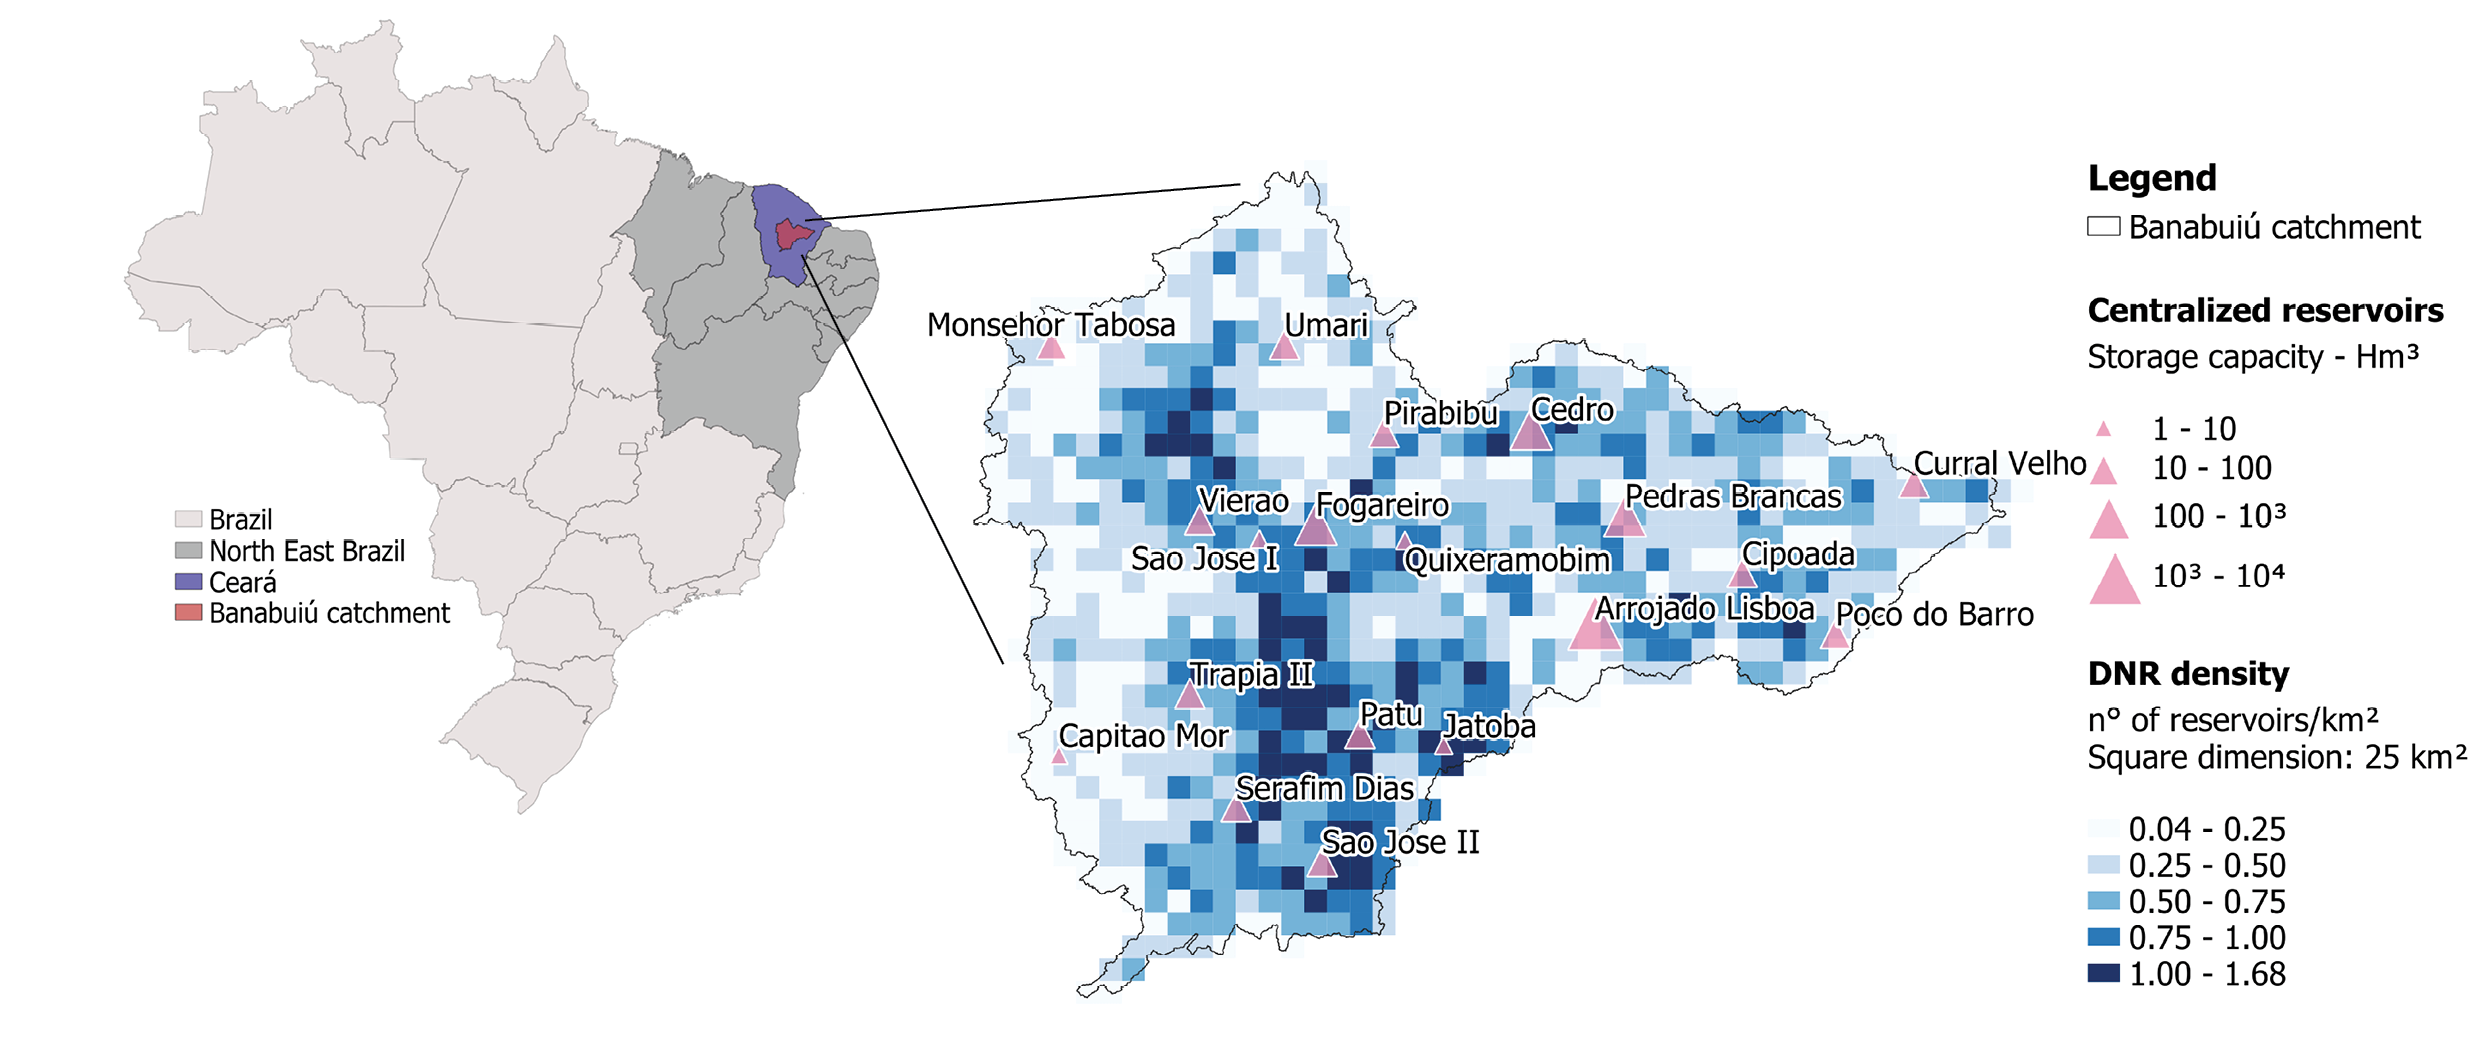
\includegraphics[width=\textwidth]{images/Figure_1.png}
 \caption{Study area framing. North-East Brazil, Ceará and Banabuiú catchment on the left. On the right, centralized reservoirs location and storage capacity, overlayed to DRN’s density in the Banabuiú basin.}
 \label{fig1}
\end{figure}

The semi-arid region of Brazil (North-East Brazil) occupies about 11\% of the Brazilian territory (1,006,654 $km^2$) and has a population of 26 million inhabitants \cite{Marengo2020}. It is a representative example of a region with a high concentration of reservoirs with great variation in size and storage capacity. North-East Brazil (NEB) has a highly irregular spatio-temporal precipitation regime, which means the region is frequently affected by intense drought events. Sixteen out of the last 25 years registered rainfall below normal in the region. In 2010 the most severe drought ever recorded started, which ended in 2018 \cite{MarengoOrsini2018,Marengo2017}. The combination of the predominance of soils and geology with low water storage capacity produces a dependency on the superficial storage of water \cite{Marengo2017,Rossato2017}. Water supply then relies on the reservoirs that regularize discharges. Their storage capacity varies from small reservoirs used on private properties to large reservoirs used for urban supply, industrial demands, and large irrigation areas (also called hydrosystems). A total of 17,083 reservoirs with surface area greater than 5 ha are located in the NEB. This system has a cumulative capacity of 707.36 billion $m^3$, according to the database from Reservoir Monitoring System of the Brazilian National Water Agency (Agência Nacional de Águas e Saneamento Básico) in 2016 \cite{Nascimento2017}. A representative example of this situation is Ceará, a 148,886 km² wide state in semi-arid Brazil, where it is estimated the presence of 105,813 reservoirs with more than 20 meters in length \cite{FUNCEME2021}. Ceará presents areas with reservoir concentration higher than 7 reservoirs per $km^2$ \cite{RibeiroNeto2022}, which greatly exceed other high concentration areas such as India (4.2 reservoirs/$km^2$) and Australia (6.1 reservoirs/$km^2$) \cite{Rabelo2021}.\\
The study area is the Banabuiú river watershed located in the state of Ceará which covers an area of approximately 19,000 $km^2$. The river network, starting from the main tributary Rio Quixeramobim, delineates the division of the basin into sub-basins and determines the distribution of the strategic reservoirs, placed along the network branches. The Banabuiú basin counts 19 monitored reservoirs with storage capacity above 1·$Hm^3$ ($10^6 m^3$) , with the biggest being Arrojado Lisboa at 1600 $Hm^3$. These reservoirs, shown in Figure~\ref{fig1}, are continuously monitored and managed by the State water agency (Water Resources Company, COGERH) and account for 2790 $Hm^3$, 93\% of the overall water storage capacity in the basin. At the same time, a cumulative 210 $Hm^3$ storage capacity is retained in approximately 10,000 small reservoirs, which constitute the DRN and are visualized together with strategic reservoirs present in the basin in Figure~\ref{fig1}. Despite their small proportion in relation to total capacity (7.1\%), small reservoirs have an important role in the water supply of small rural communities, whose needs are not met by the large hydrosystems, as the water stored in small reservoirs enables local distribution. In the region, most of the small reservoirs aim to meet the water necessities of subsistence farmers only in the short term (6-8 months in the dry season). The small reservoirs also serve as sediment detention basins, retaining a considerable amount of sediment generated within the catchment and extending the life-time of larger ones located downstream \cite{Mamede2018}. However, their presence can reduce the potential yield of strategic reservoirs which may determine a lower possibility to store and distribute water during droughts \cite{Krol2011}. 

\subsection{DRN capacity estimation}\label{sec:drncap}

%Table 1
\begin{table}
 \caption{Repartition of the reservoirs composing the Dense Reservoir Network in the Banabuiú basin.}\label{tab1}
 \centering
 \begin{tabular*}{\textwidth}{m{1.5cm} m{2cm} m{2cm} m{2cm} m{2.3cm} m{2.3cm}}
 \hline
  Reservoir class & Storage volume - upper limit &  Number of reservoirs & Percentage of reservoirs & Class cumulative storage volume & Class cumulative storage volume\\
  & [$m^3$] & & [\%] & [$Hm^3$] & [\%]\\
 \hline
1	& 5000	 & 6977	&	67.4	 &	7.2  &	3.4\\
2	& 25000	 & 1787	&	17.3	 &	21	 & 10\\
3	& 50000	 & 546	&	5.3	 &	20	 & 9.4\\
4	& 100000	 & 447	&	4.3	 &	32	 & 14.8\\
5	& 500621	 & 598	&	5.8	 &	130	 & 62.4\\
 \hline
Total &	-	& 10355 &	100	 &  210.2 &	100\\
 \end{tabular*}
\end{table}

The capacity of the DRN-component reservoirs is needed to represent the network in the hydrological model.  Neither capacity nor surface area were available. Therefore, a capacity estimation has been obtained starting from the Joint Research Center’s (JRC) Global Surface Water Explorer, which provides a worldwide database of surface water imagery \cite{Pekel2016}. The maximum water extent raster, which maps the maximum extent of water bodies in an area, was connected with the locations of the DRN (surveyed in \citeA{FUNCEME2021}), associating each reservoir location to the nearest water body through a nearest neighbor algorithm. In this way, 10,355 small reservoirs had their maximum area associated. Reservoirs without a corresponding water body in JRC’s representation (approximately 7,000) were left out of the final configuration, represented in Figure~\ref{fig1} and summarized in Table~\ref{tab1}. The causes of them not being represented may lay in their small size, which is difficult to be detected and validated through JRC’s satellite images, or in inaccuracies in the survey operated by \citeA{FUNCEME2021}, where small topographic depressions could have been erroneously interpreted as reservoirs, such as natural depressions in lowlands and depressions close to roads. The capacity of each reservoir (V) was then obtained from the area (A) through Molle’s equation (Equation 1), where $\alpha$ and K parameters are equal to average values of 2.7 and 1,500 respectively, as used in literature in North-East Brazil \cite{Mamede2018,Mamede2012,Molle1994}. In this study, a reservoir is considered small when its capacity is lower or equal to 500,000 $m^3$ (0.5 $Hm^3$), since this was the highest storage capacity of the unmonitored reservoirs in the basin.
\begin{linenomath*}
	\begin{equation}
	V = K \cdot (\frac{A}{\alpha\cdot K})^\frac{\alpha}{\alpha -1}
	\end{equation}
\end{linenomath*}

\subsection{Modeling approach}\label{sec:model}
\subsubsection{WASA-SED model}
The model selected to model the Banabuiú river basin is WASA-SED (Water Availability in Semi-Arid environments-SEDiments), which has been developed within the joint Spanish-Brazilian-German research project SESAM (Sediment Export from Semi-Arid Catchments: Measurement and Modelling) and utilized to simulate North-East Brazil’s conditions \cite{Guntner2002,Guntner2004,Mueller2010}. The model simulates the runoff and erosion processes at meso-scale, for domains ranging from several hundreds to thousands of square kilometers. It uses a hierarchical top-down disaggregation scheme, dividing each sub-basin of the model into landscape units (based on the Soil and Terrain Digital Database (SOTER) concept \cite{Oldeman1993}), represented by multiple terrain components (defined by slope-gradient, length, soil and soil-vegetation components). The hydrological module is fully described in \citeA{Guntner2002} and \citeA{Guntner2004}, implementing for example equations to account for interception losses, evaporation and transpiration (modified Penman-Monteith approach \cite{Shuttleworth1985}) and for infiltration (Green-Ampt approach \cite{Green1911}) and other soil and vegetation related processes. The model can simulate both medium and large  centralized strategic reservoirs and small diffuse networks of reservoirs \cite{Guntner2004}. The user manual, the link to the source code and other useful sources can be found at \url{github.com/TillF/WASA-SED}. Detailed WASA-SED model parameterization for Banabuiú river basin was carried out by \citeA{Costa2013}, and adopted in this work.

\subsubsection{Small reservoirs representation}
The modeling approach to the reservoirs needs to classify them into strategic and small reservoirs, according to location and size \cite{Guntner2004}. The strategic reservoirs listed in Table~\ref{tab1} are individually parameterized in WASA-SED, also providing their daily regulated discharge time series. Their water balance is calculated explicitly and individually for each reservoir. Due to the uncontrolled and unmonitored nature of small reservoirs composing the DRN, not enough information is available concerning dam building, location, size and water use. They are grouped into 5 storage capacity classes and the water balance is computed for a hypothetical reservoir with mean characteristics, representative of each class and sub-basin. The water storage volume is then given by the product of the water storage of the representative reservoir by the total number of reservoirs from that class within a sub-basin. The generated runoff of the sub-basin is distributed among the reservoir classes through a cascade routing scheme starting from the lowest class to the highest, using a weighting factor computed as a ratio between the runoff contributing area of that reservoir class and the sub-basin area \cite{Mamede2018}. A detailed description of the calculation of water fluxes through the classes of reservoirs can be found in \citeA{Mamede2008}, while equations and other information about the hydrological and reservoir module can be found in \citeA{Guntner2002}.

\subsubsection{Calibration and validation}
Calibration was focused on the “scaling factor” parameter, which modifies the soil saturated hydraulic conductivity, which is the most sensitive parameter \cite{Guntner2002,WASA-SEDManual2021}. The calibration was carried out automatically following the sub-basins routing path of the model from upstream to downstream, testing a set of 35 values on each sub-basin (ranging from 0.2 to 7). For each run, five model performance indexes were computed (R2, NSE, KGE, PBIAS and NRMSE) comparing the modeled volume time series for the sub-basin’s strategic reservoir (or the direct downstream one in case the sub-basin did not present one itself) with the observed one. The performance indexes were selected based on recent usage in hydrological modeling \cite{Marahatta2021,Knoben2019,Uniyal2019}. The parameter that would produce the best performance was selected. The model was calibrated with 70\% of the series, running it from 1980 to 2006, it was then validated on the remaining 30\% of the series, from 2007 to 2018. Wet, normal and dry years were well represented in both the selected periods (calibration and validation) of the gauges. Therefore, the high inter-annual streamflow variability (CV greater than 1) was taken into account for both calibration and validation periods.

\subsubsection{Scenarios generated and used in the analyses}\label{sec:scenarios}

%Figure 2
\begin{figure}
 \noindent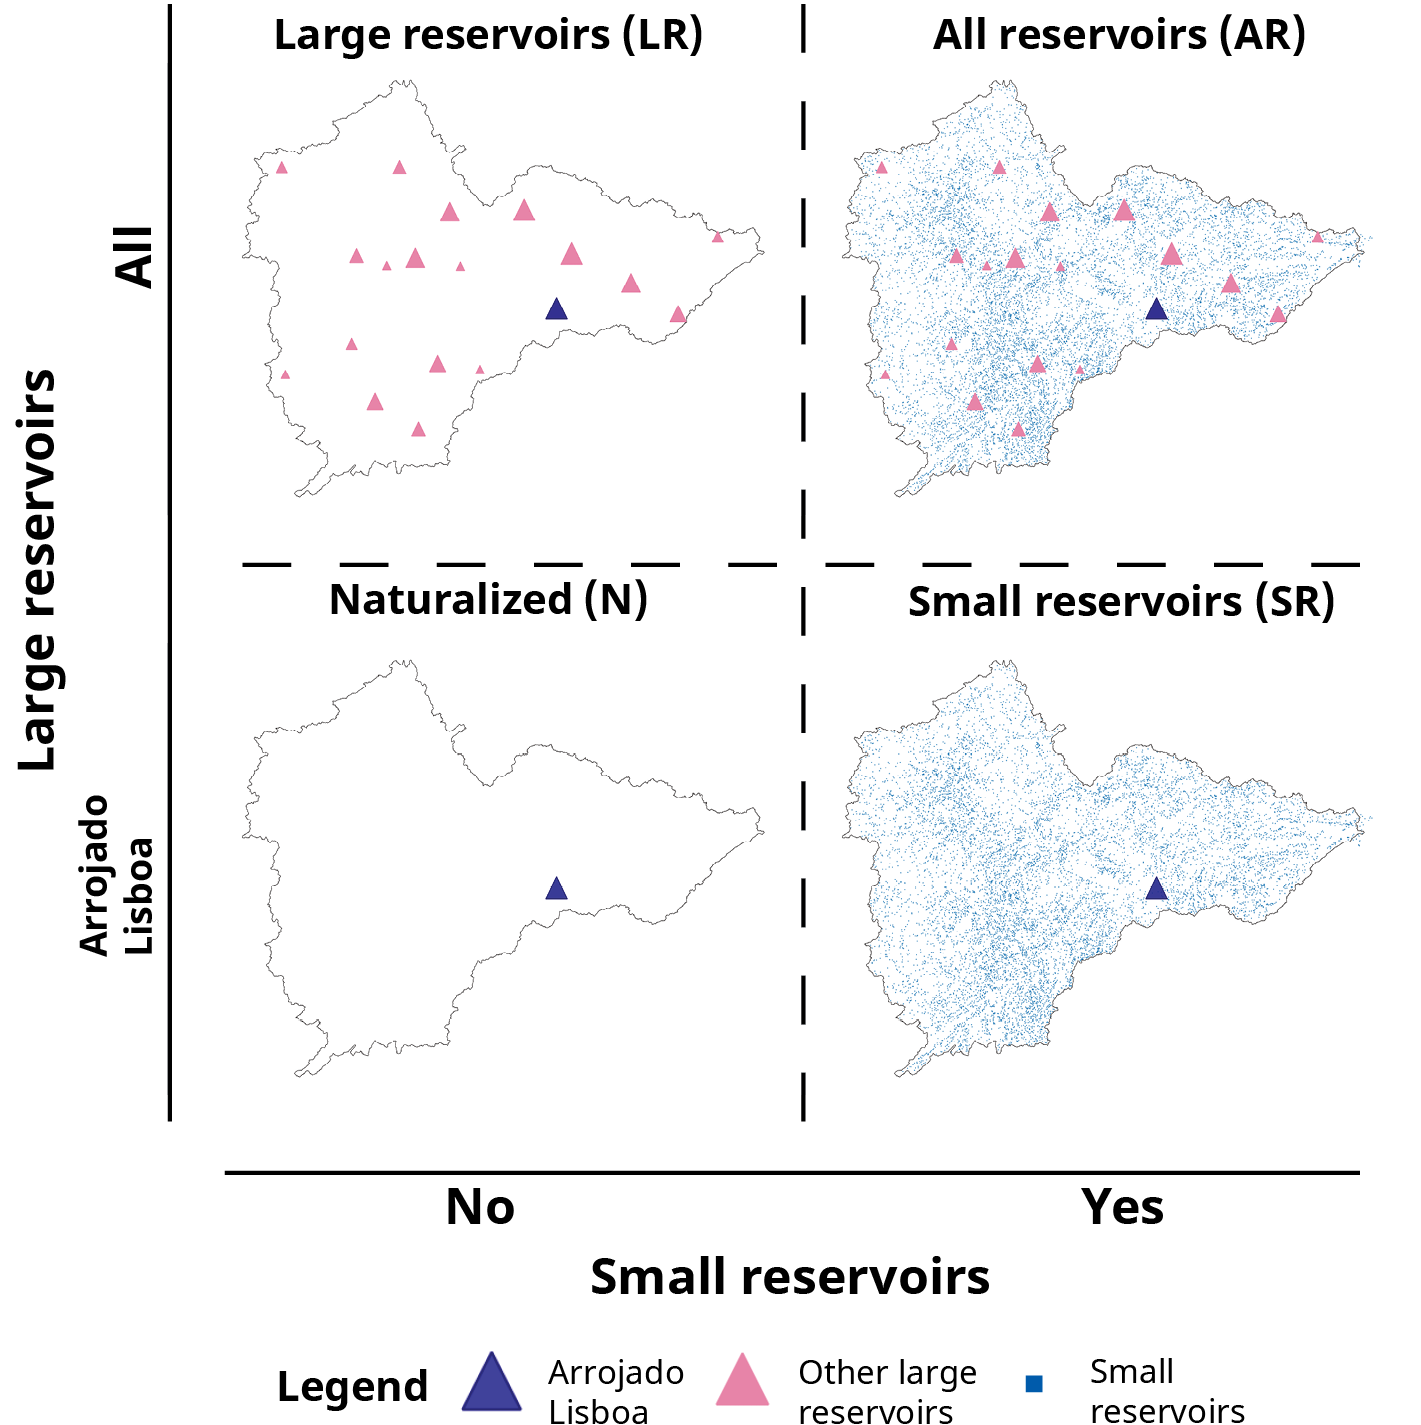
\includegraphics[width=\textwidth]{images/Figure_2.png}
 \caption{Visualization of the modeled scenarios design: Large Reservoirs (LR), centralized reservoirs only; All Reservoirs (AR), centralized reservoirs and DRN; Naturalized (N), Arrojado Lisboa only; and Small Reservoirs (SR), DRN and Arrojado Lisboa only.}
 \label{fig2}
\end{figure}

Four different configurations were modeled, as visualized in Figure~\ref{fig2}. The All Reservoirs (AR) configuration represents the real condition, with the co-existence of the small and large reservoirs. The dense reservoir network was removed to keep only large reservoirs in the Large Reservoirs (LR) scenario. These were also removed to obtain two scenarios not influenced by them: Small Reservoirs (SR), representing only small reservoirs and Arrojado Lisboa, and Naturalized (N), representing only Arrojado Lisboa. The only reservoir present in all the scenarios is Arrojado Lisboa, the most downstream, used as a reference for the comparisons in all the analyses. The differences between AR and LR scenarios have been explored in order to assess the effects of the DRN on droughts’ evolution in time and space. N and SR scenarios have been useful to explore the DRN effects without the influence of large reservoirs.

\subsection{Drought analyses}\label{sec:analyses}
To effectively consider the effects that the existence of a DRN produces on drought evolution, two domains have been considered: time, to address impacts on frequency and duration of drought, and space, to include the effects on water distribution. This dual aspect has been analyzed through the Drought Cycle Analysis (\ref{sec:DCA}) \cite{RibeiroNeto2022} and the Downstreamness Analysis (\ref{sec:dwn}) \cite{VanOel2011}. The different scenarios created through the WASA-SED model will be compared with these methods in order to estimate the influence of the DRN on hydrological drought evolution and propagation.

\subsubsection{Drought Cycle Analysis}\label{sec:DCA}

%Figure 3
\begin{figure}
 \noindent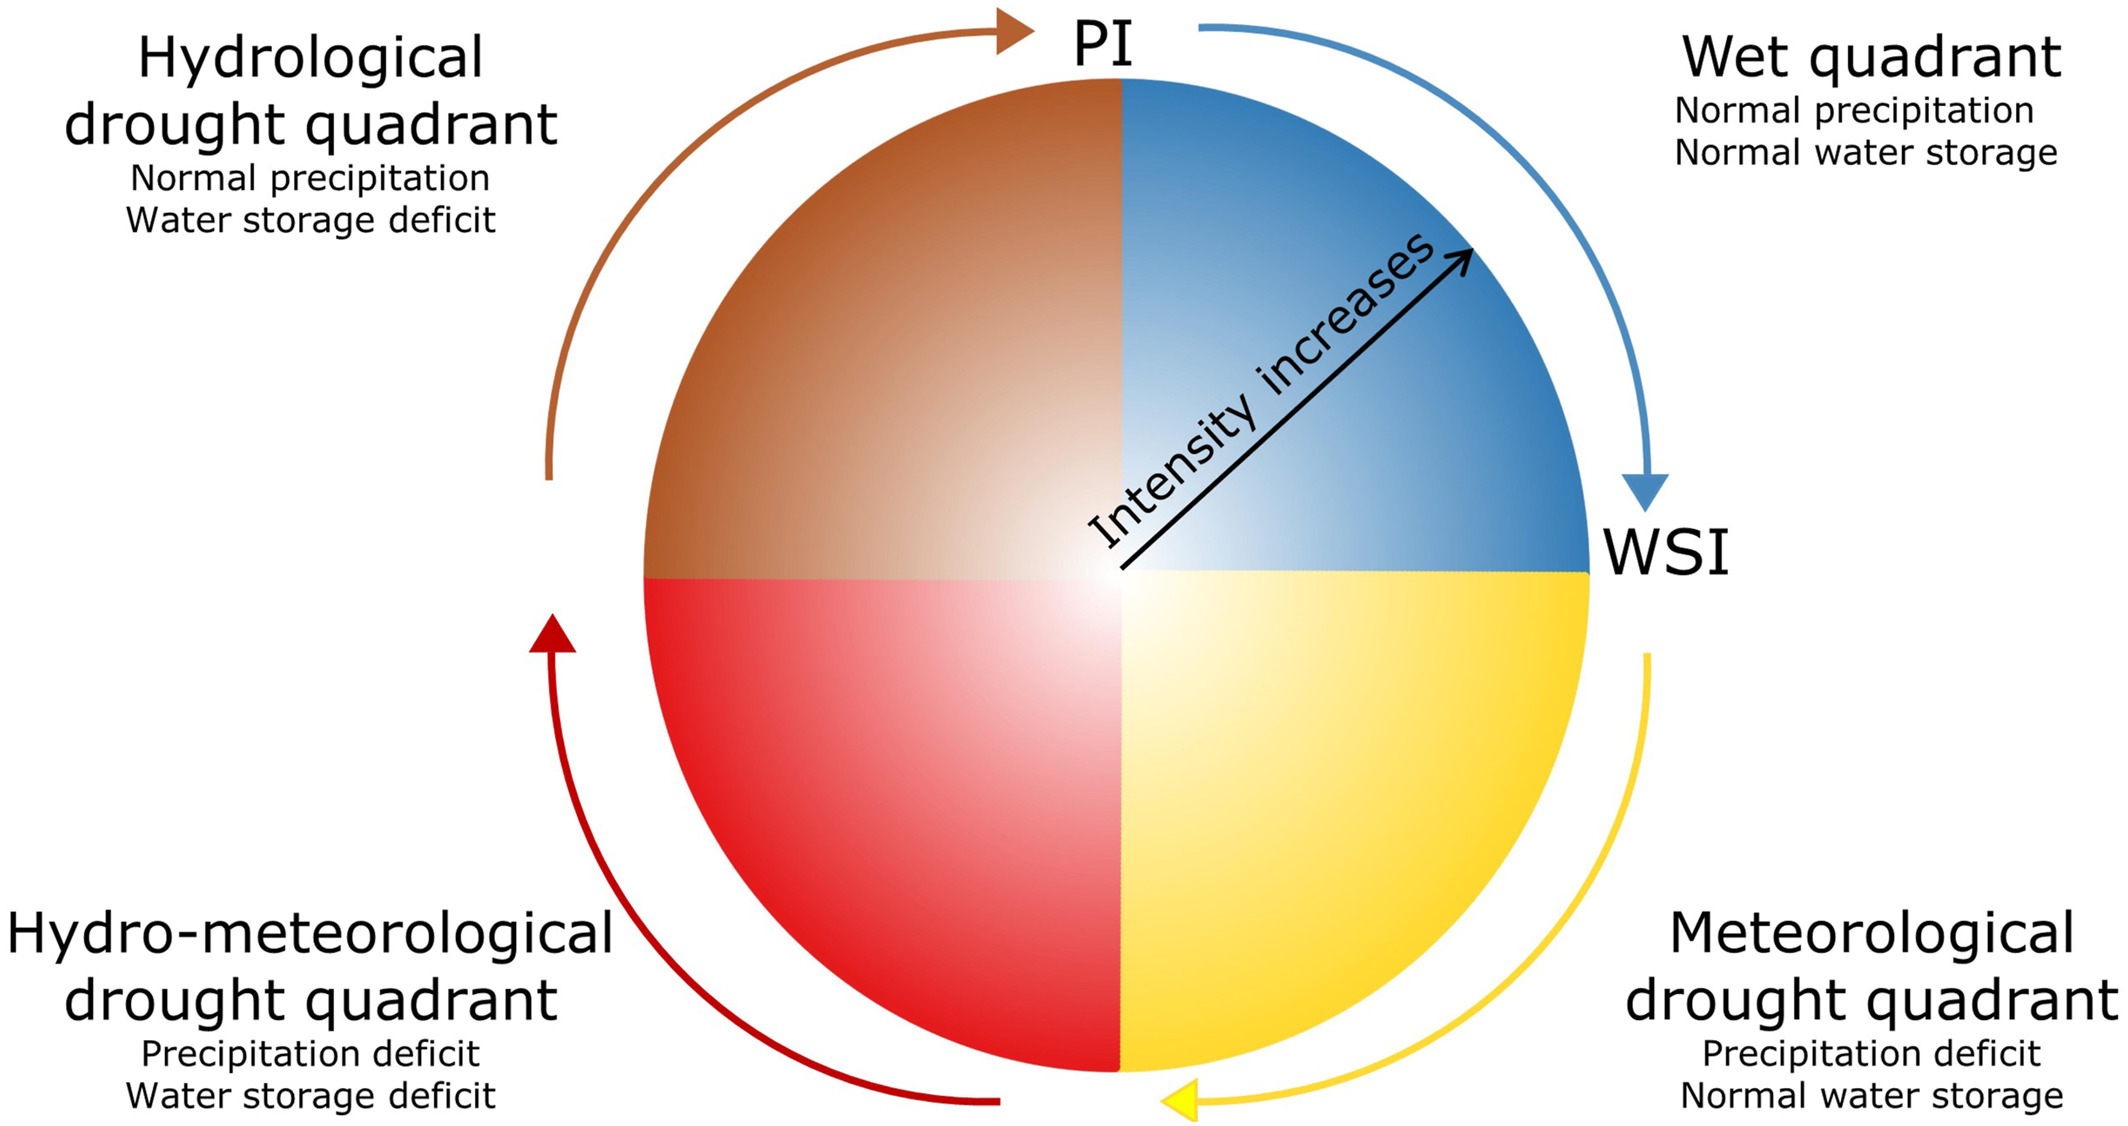
\includegraphics[width=\textwidth]{images/Figure_3.jpg}
 \caption{Graphical representation of the Drought Cycle Analysis, from \citeA{RibeiroNeto2022}. WSI: Water Storage Index, PI: Precipitation Index.}
 \label{fig3}
\end{figure}

The Drought Cycle Analysis (DCA) is a recent method proposed by \citeA{RibeiroNeto2022}, based on a combination of precipitation and hydrological indexes. It classifies drought events into four possible stages. The indexes values are positioned in quadrants in the coordinate system shown in Figure~\ref{fig3}, with a hue and tone variation scheme to represent the intensity of drought event as well as its classification, respectively.\\
The first quadrant is the non-occurrence of drought: positive values of both Precipitation Index (PI, vertical axis) and Water Storage Index (WSI, horizontal axis). The next quadrant indicates meteorological drought, when there is a precipitation deficit (PI < 0) but it has not yet affected water storage (WSI > 0). In the third quadrant, hydro-meteorological drought takes place, which is the coexistence of meteorological and hydrological drought. Water storage is affected by the persistence of meteorological drought and reservoirs deplete consistently. Therefore, both indexes reach negative values. The final quadrant is the "Hydrological drought quadrant", which is characterized by the persistence of hydrological drought (WSI < 0) after the end of meteorological drought (PI > 0).\\
Standardized indexes are used as they allow a better division in the quadrants proposed: negative values of the index mean a scarcity condition, while positive values mean the opposite. In order to compute the analysis, the Precipitation Index and the Water Storage Index can be chosen from the many available. The same procedure as \citeA{RibeiroNeto2022} has been followed. The Standardized Precipitation Index (SPI) over 12 months (SPI-12) has been utilized as PI (WMO, 2012). The Volume Deviation (VD) of Arrojado Lisboa reservoir (the largest and most downstream one) is utilized as a proxy for the water storage of the study area (WSI). VD is an index considering the deviation of a reservoir’s volume from the half of its total capacity. It can thus vary from -1 to 1, with positive values meaning a volume higher than half of the total capacity and negative values meaning the opposite. The indexes are computed at monthly resolution, the results of the Drought Cycle Analysis will then have a monthly resolution themselves. This method considers a meteorological index for monitoring droughts (the vertical axis of the drought wheel) and information directly related to the impact that this can cause (the horizontal axis of the drought wheel). This allows us to identify drought events defined as disasters related to the exceptional lack of water that is prejudicial for human activities or environmental demands. Further details and discussion on this method can be found in \citeA{RibeiroNeto2022}.

\subsubsection{Downstreamness analysis}\label{sec:dwn}
The downstreamness concept aims to analyze the availability and distribution of water resources in a river basin, first introduced in \citeA{VanOel2009} and successively developed and used to analyze basin closure and to diagnose hydrological droughts \cite{VanOel2011,VanOel2018,HvanLangen2021}. The downstreamness of a location ($D_{x}$), for example a reservoir’s dam outlet, is the ratio of its upstream catchment area ($A_{up}$) to the entire river basin area ($A_{tot}$) (Equation 2). Higher the index, the more downstream the location x will be.\\

%Equation 2, 3, 4
\begin{linenomath*}
 \begin{equation}\label{Dx}
 D_{x} = \frac{A_{up,x}}{A_{tot}} \cdot 100 [\%]
 \end{equation}
\end{linenomath*}
\begin{linenomath*}
 \begin{equation}\label{DSC}
 D_{SC} = \frac{\sum_{x=1}^{n} SC_{x}D_{x}}{\sum_{x=1}^{n} SC_{x}}
 \end{equation}
\end{linenomath*}
\begin{linenomath*}
 \begin{equation}\label{DSV}
 D_{SV} = \frac{\sum_{x=1}^{n} SV_{x}D_{x}}{\sum_{x=1}^{n} SV_{x}}
 \end{equation}
\end{linenomath*}

The downstreamness of a basin’s function (like water availability or water demand) is defined as the downstreamness-weighted integral of that function divided by its regular integral \cite{VanOel2011}. Higher the index, more downstream the distribution of the variable will be. In this study, the functions considered are the basin’s storage capacity (Equation 3) and the basin’s stored volume (Equation 4). Each reservoir’ storage capacity ($SC_{x}$) and stored volume ($SV_{x}$) are utilized to find two monthly scaled indicators of the distribution of these variables in the basin ($D_{SC}$ and $D_{SV}$ respectively). To extract reservoirs’ $A_{up}$ their positions were overlaid to the flow accumulation raster obtained from the area’s Digital Elevation Model (DEM). $A_{tot}$ is taken at the basin outlet.  An assumption was made in order to be able to handle the DRN keeping the spatial information on its reservoirs: the number of reservoirs was kept the same across all the years considered. This approximation means that considerations about the effects of the evolution of the DRN in time can not be made, but at the same time it makes the analysis on the effects more sound because it reduces the growing uncertainty about the number and location of small reservoirs in the past, since a mapping of the small reservoirs across the years is not available.\\
The information needed to compute $D_{SC}$ was available or made available for both strategic (from FUNCEME database: \url{funceme.br/hidro-ce-zend/}) and small reservoirs (from the operations explained in \ref{sec:drncap}). $D_{SV}$ was computed using the modeled reservoirs volume time series. For the strategic reservoirs, the model output could be used untouched. For the DRN, the WASA-SED model computes the small reservoirs volumes for the whole catchment after grouping them by reservoir size classes (one value for the whole catchment and each reservoir size class). These values were returned to an average value dividing by the number of small reservoirs in the respective sub-basin and class. The result was assigned to each reservoir of that sub-basin and class, as their $SV_{x}$.

\section{Results}
\subsection{Model calibration and validation results}

%Table 2
\begin{table}
 \caption{Mean performance of WASA-SED model after calibration, validation and on the whole time series}\label{tab2}
 \centering
 \begin{tabular}{c c c c}
 \hline
  Index  & Calibration period & Validation period & Whole period\\
  & (1980 $-$ 2006) & (2007 $-$ 2018) & (1980 $-$ 2018)\\
 \hline
	$R^2$ & 0.598  & 0.600  & 0.519  \\
	NSE   & 0.0497 & 0.360  & 0.271  \\
	PBIAS & 7.853  & -3.881 & -1.523 \\
	KGE   & 0.462  & 0.572  & 0.674  \\
	NRMSE & 0.257  & 0.239  & 0.246  \\
 \hline
 \end{tabular}
\end{table}

From approximately 945 runs that were performed and evaluated an optimal configuration of parameters was selected. Table~\ref{tab2} shows the calibration, validation and whole time series performances averaged over the sub-basins.

\subsection{Drought Cycle Analysis}
\textbf{Meteorological Drought}

%Figure 4
\begin{figure}
 \noindent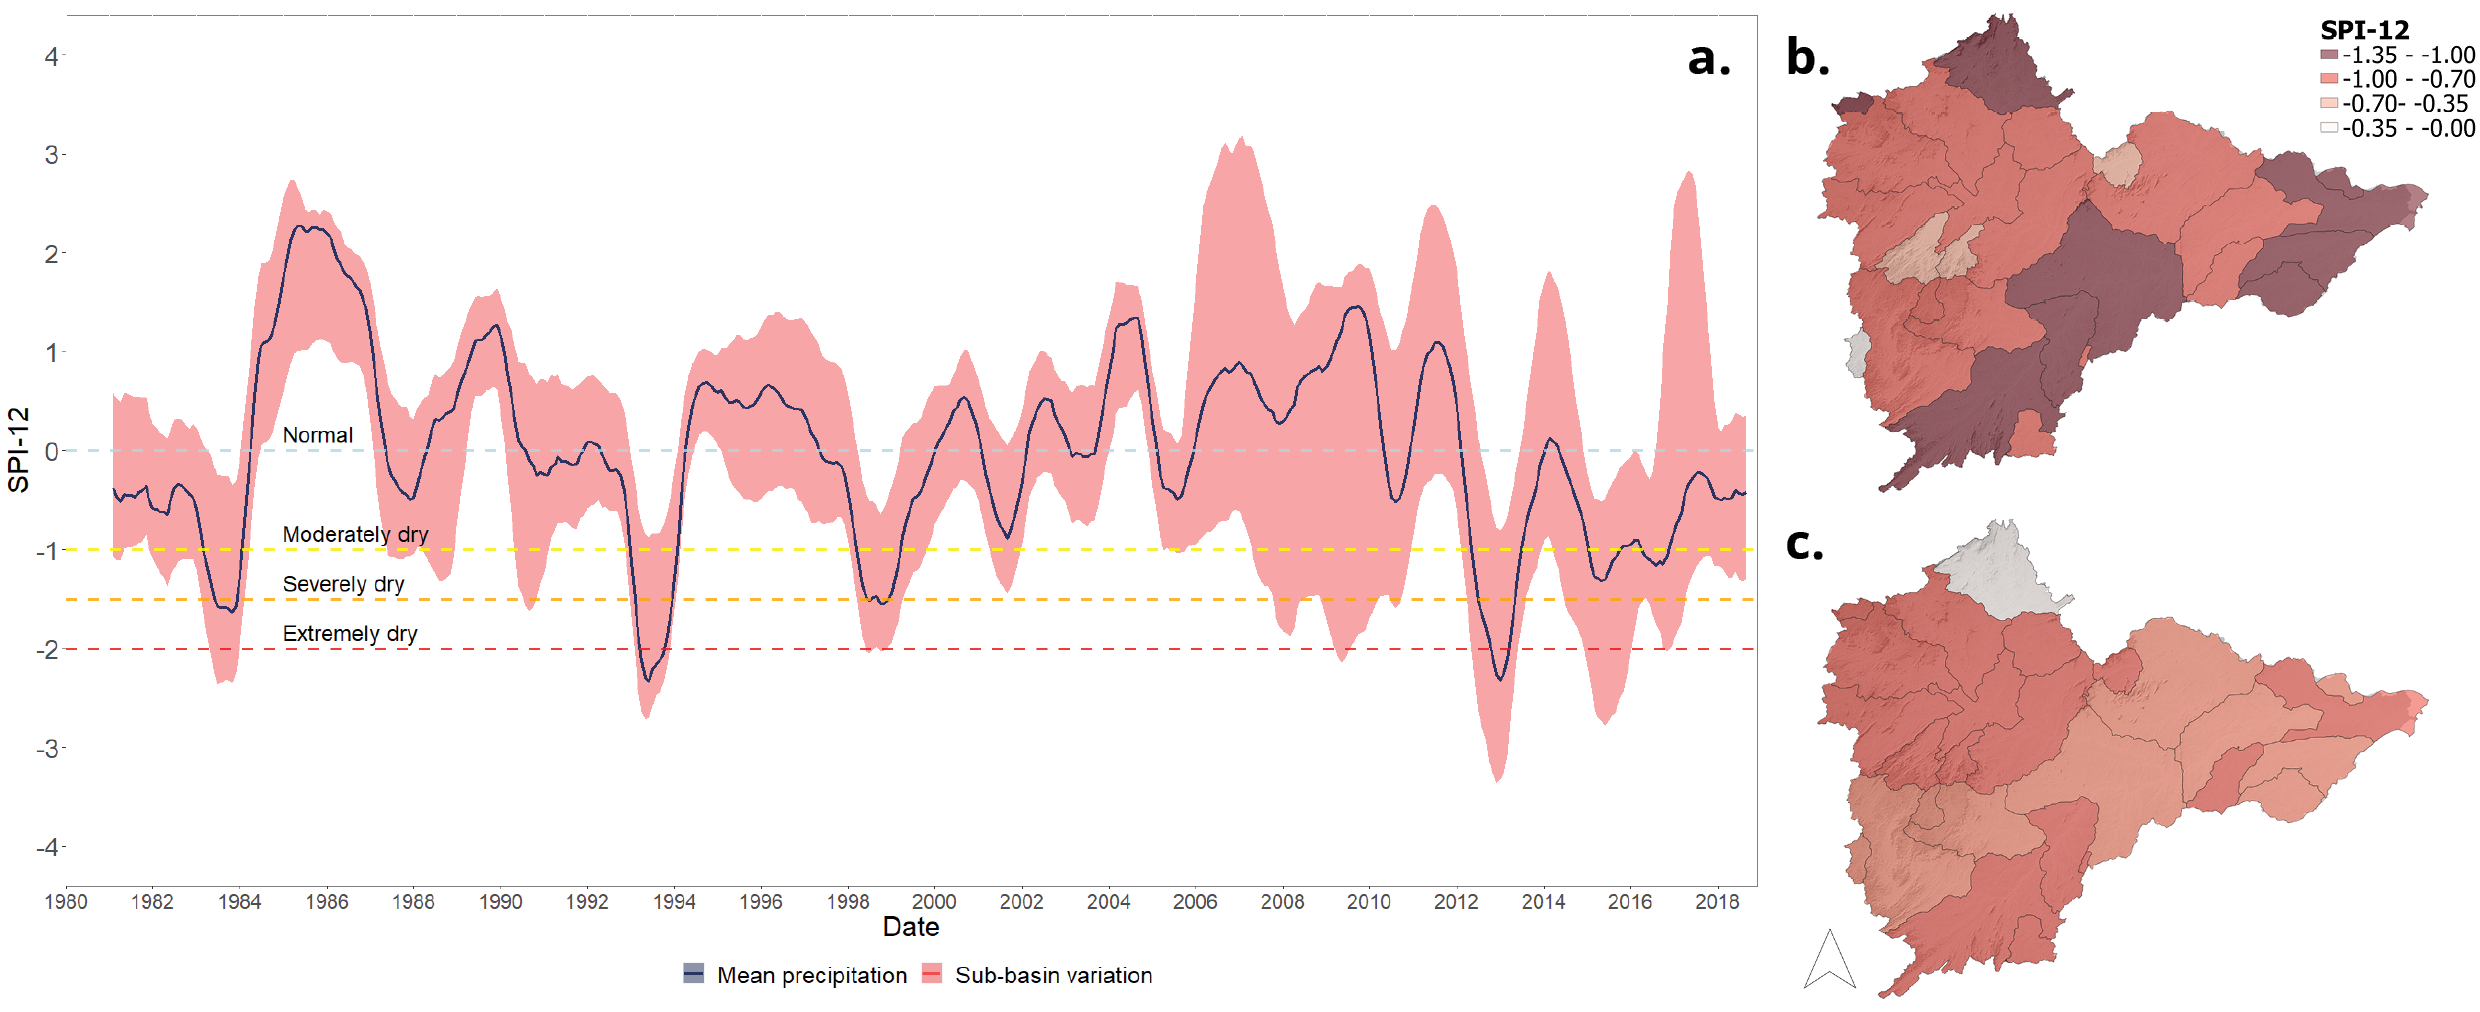
\includegraphics[width=\textwidth]{images/Figure_4.png}
 \caption{SPI-12 visualization. a.) 6-months moving average of the SPI-12 computed on the basin’s average precipitation and variability spectrum across the sub-basins. Spatial distribution of  SPI-12 in Banabuiú watershed sub-basins averaged for b.) 1992-1993 drought and c.) 2012-2018 drought.}
 \label{fig4}
\end{figure}

The monthly SPI-12 computed for each sub-basin helped identify the periods of meteorological droughts (Figure~\ref{fig4}). Results for the Banabuiú basin show the SPI-12 index consistently below 0 after 2012. Therefore, the region can be considered in a meteorological drought condition from 2012 until 2018, when the available precipitation time series ends. The most dry periods are 1992-1993 and 2012-2018, with mean SPI-12 surpassing -2. The gained knowledge on the basin’s meteorological drought period has been used to better interpret hydrological drought.

\textbf{Hydrological Drought}

%Figure 5
\begin{figure}
 \noindent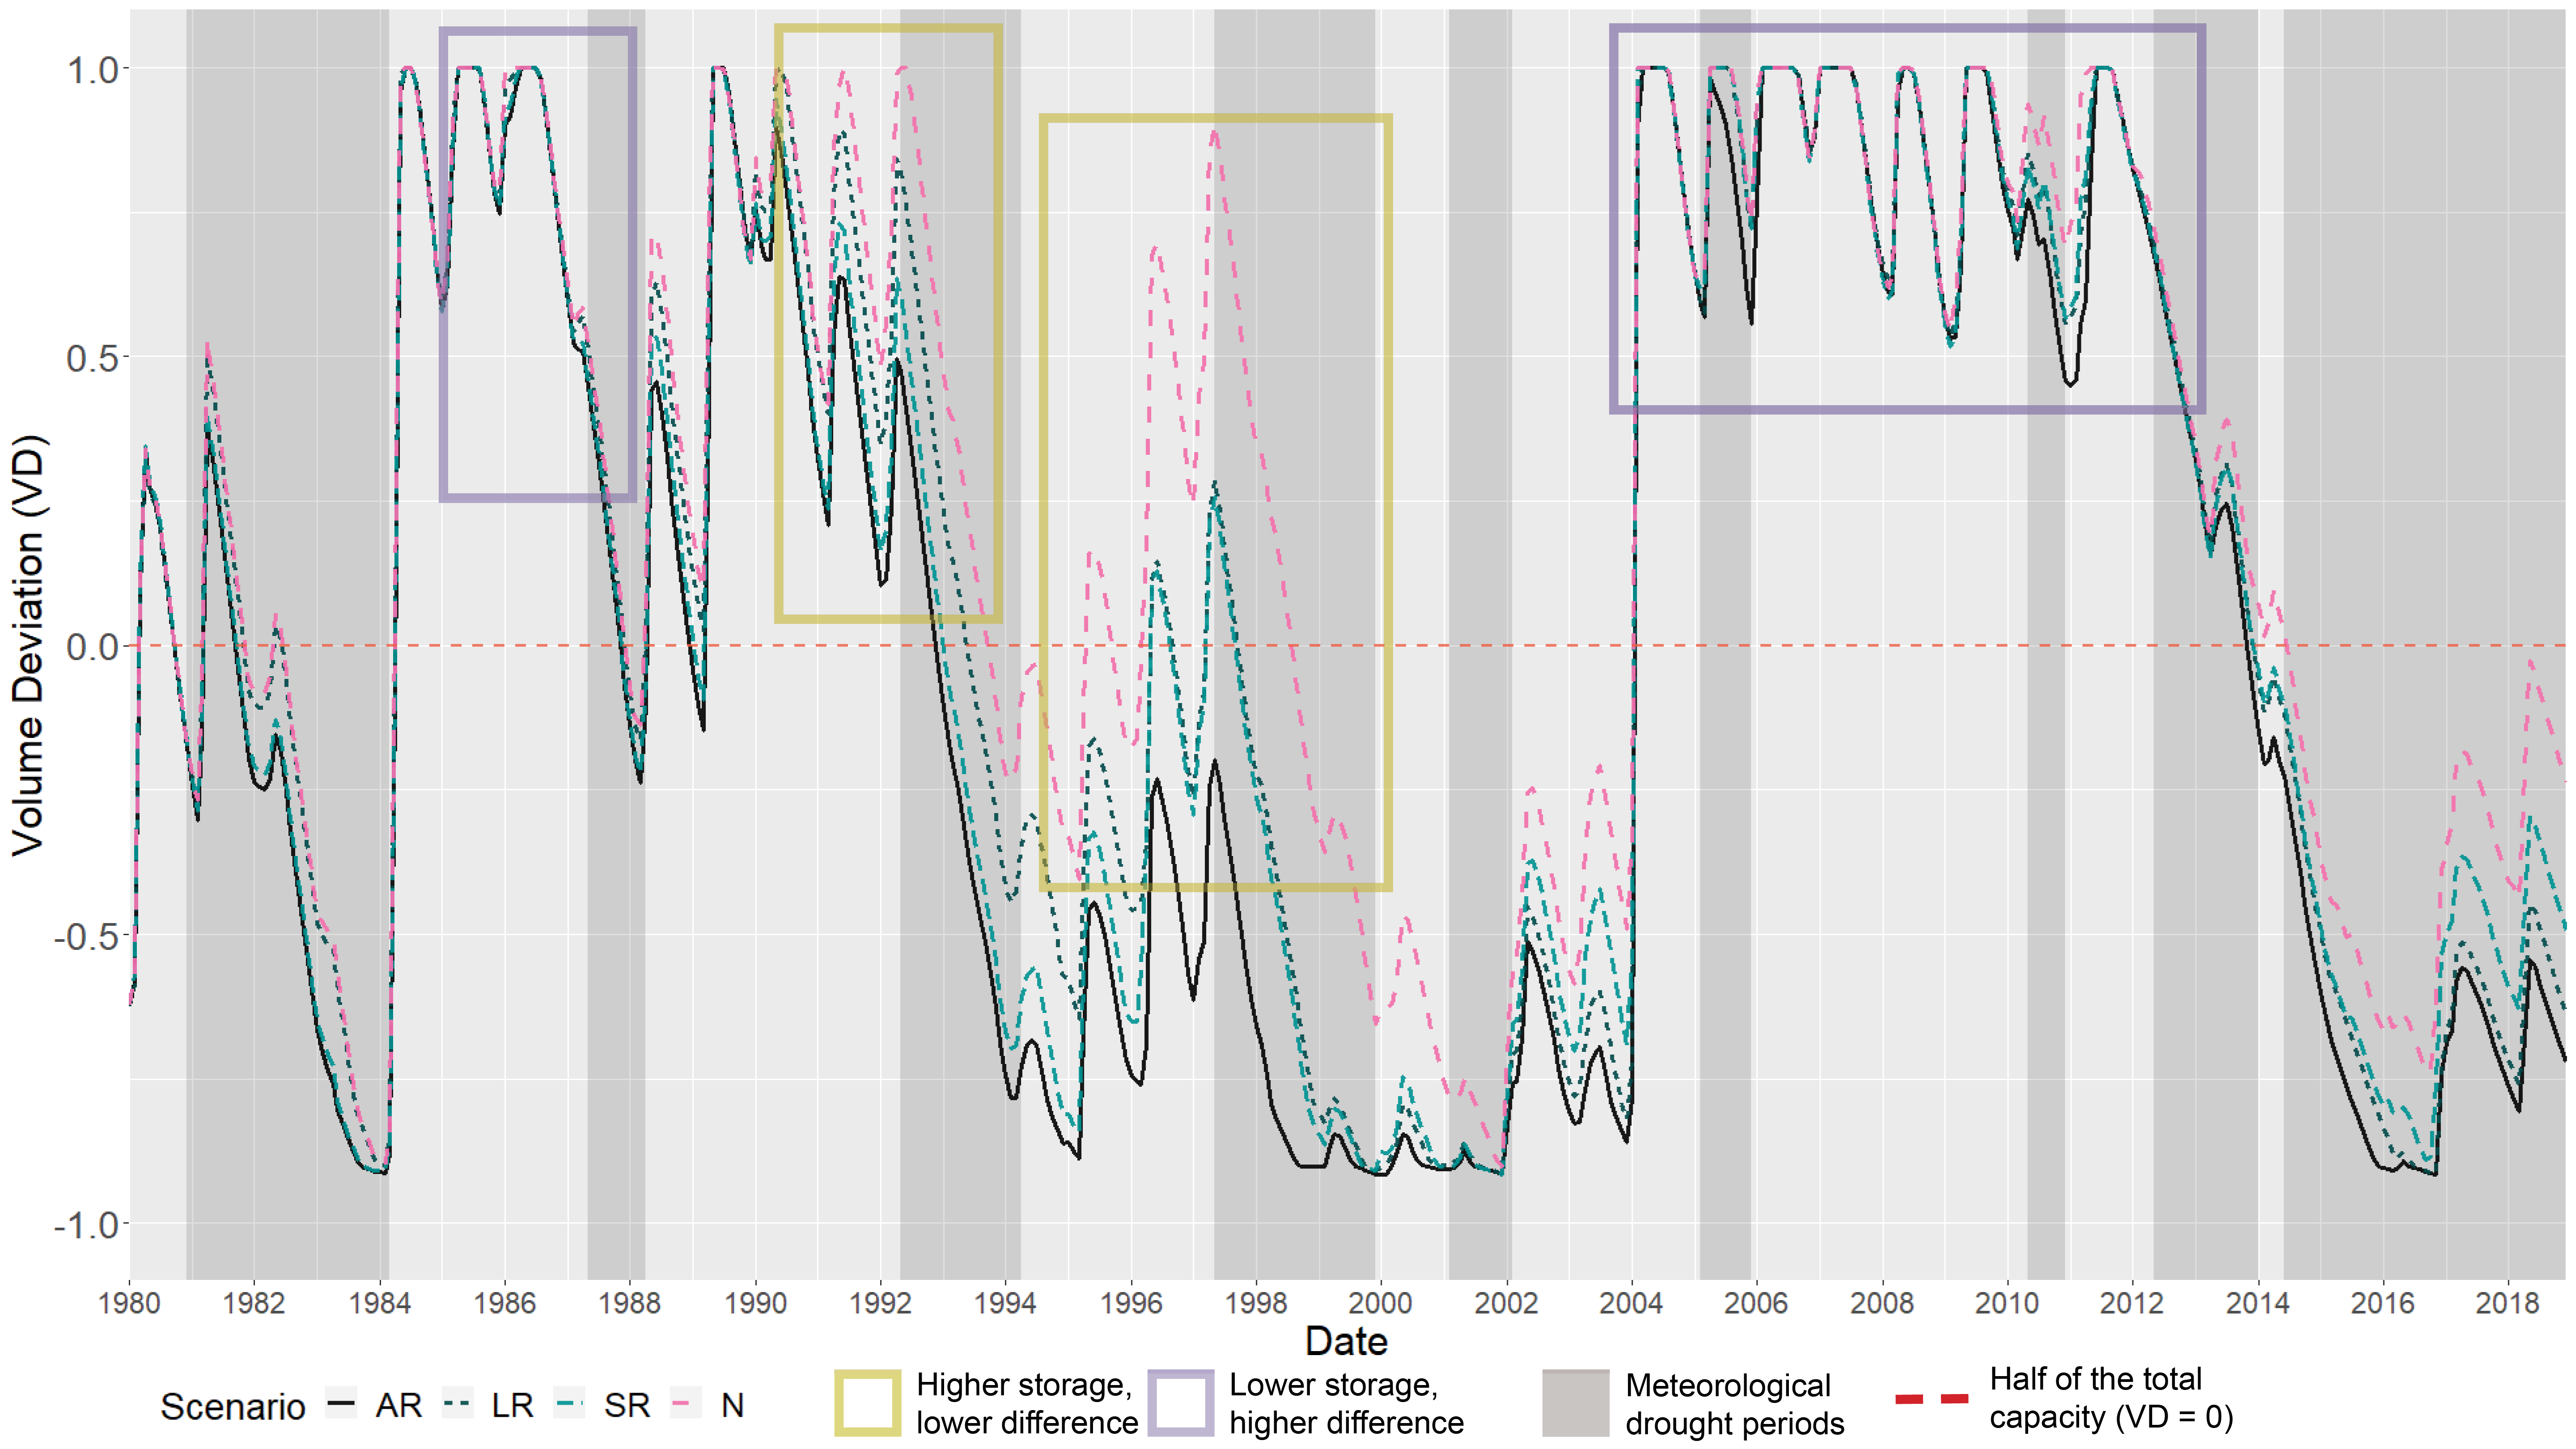
\includegraphics[width=\textwidth]{images/Figure_5.png}
 \caption{Volume Deviation visualization for all modeled scenarios. Different relationships between storage conditions and the DRN effect are indicated.}
 \label{fig5}
\end{figure}

In Figure~\ref{fig5} the Volume Deviation (VD) of Arrojado Lisboa in the four scenarios is shown. The shaded areas are periods of meteorological drought in the basin. It can be observed how the volume decreases in these periods, after which the index tends to increase. Comparing AR and LR scenarios, it is clear that the presence of the DRN has multiple influences on Arrojado Lisboa’s volume. Before the meteorological drought periods the water stored is higher without the network. This reflects afterwards, in a slower transition towards reservoirs’ depletion condition (e.g. 1992, 1997). Thus, the presence of the DRN accelerated the transition towards hydrological droughts. During and between drought events (e.g. 1994-1997, 1999-2001 and 2014), the reservoir recharge is slower by an average of 25\% in the presence of the DRN. This DRN-driven lower drought recovery leads the reservoir to be more vulnerable to multiple subsequent meteorological drought events. Removing the other large reservoirs (SR and N scenarios), the network’s effects are enhanced, with a higher difference between the two scenarios and an evident improved ability to reservoir recharge in the Naturalized scenario, as between 1996 and 2002.\\
Depending on the storage condition in which the large reservoirs are at the beginning of the meteorological droughts, the DRN effects are found at different magnitudes (Figure~\ref{fig5}). When the large reservoir is full or near the maximum capacity (VD $\geq$ 0.75) the difference between AR and LR scenarios is negligible, while with VD lower than 0.75 the difference becomes more visible. This suggests that when a meteorological drought happens, the existence of a DRN will enhance the drought effects on the reservoir more if the large reservoir is in depleted condition than it would do if the reservoir would have been full. In other words, DRN may enhance hydrological droughts' impacts when the basin is in a dry condition. A greater impact from DRN in dry conditions was found also in \citeA{Rabelo2021}. Having a better knowledge of this phenomenon may help the implementation of short term drought preparedness measures when the reservoirs are below a threshold (e.g. 75\% of the maximum capacity).

\textbf{Drought phases}

%Figure 6
\begin{figure}
 \noindent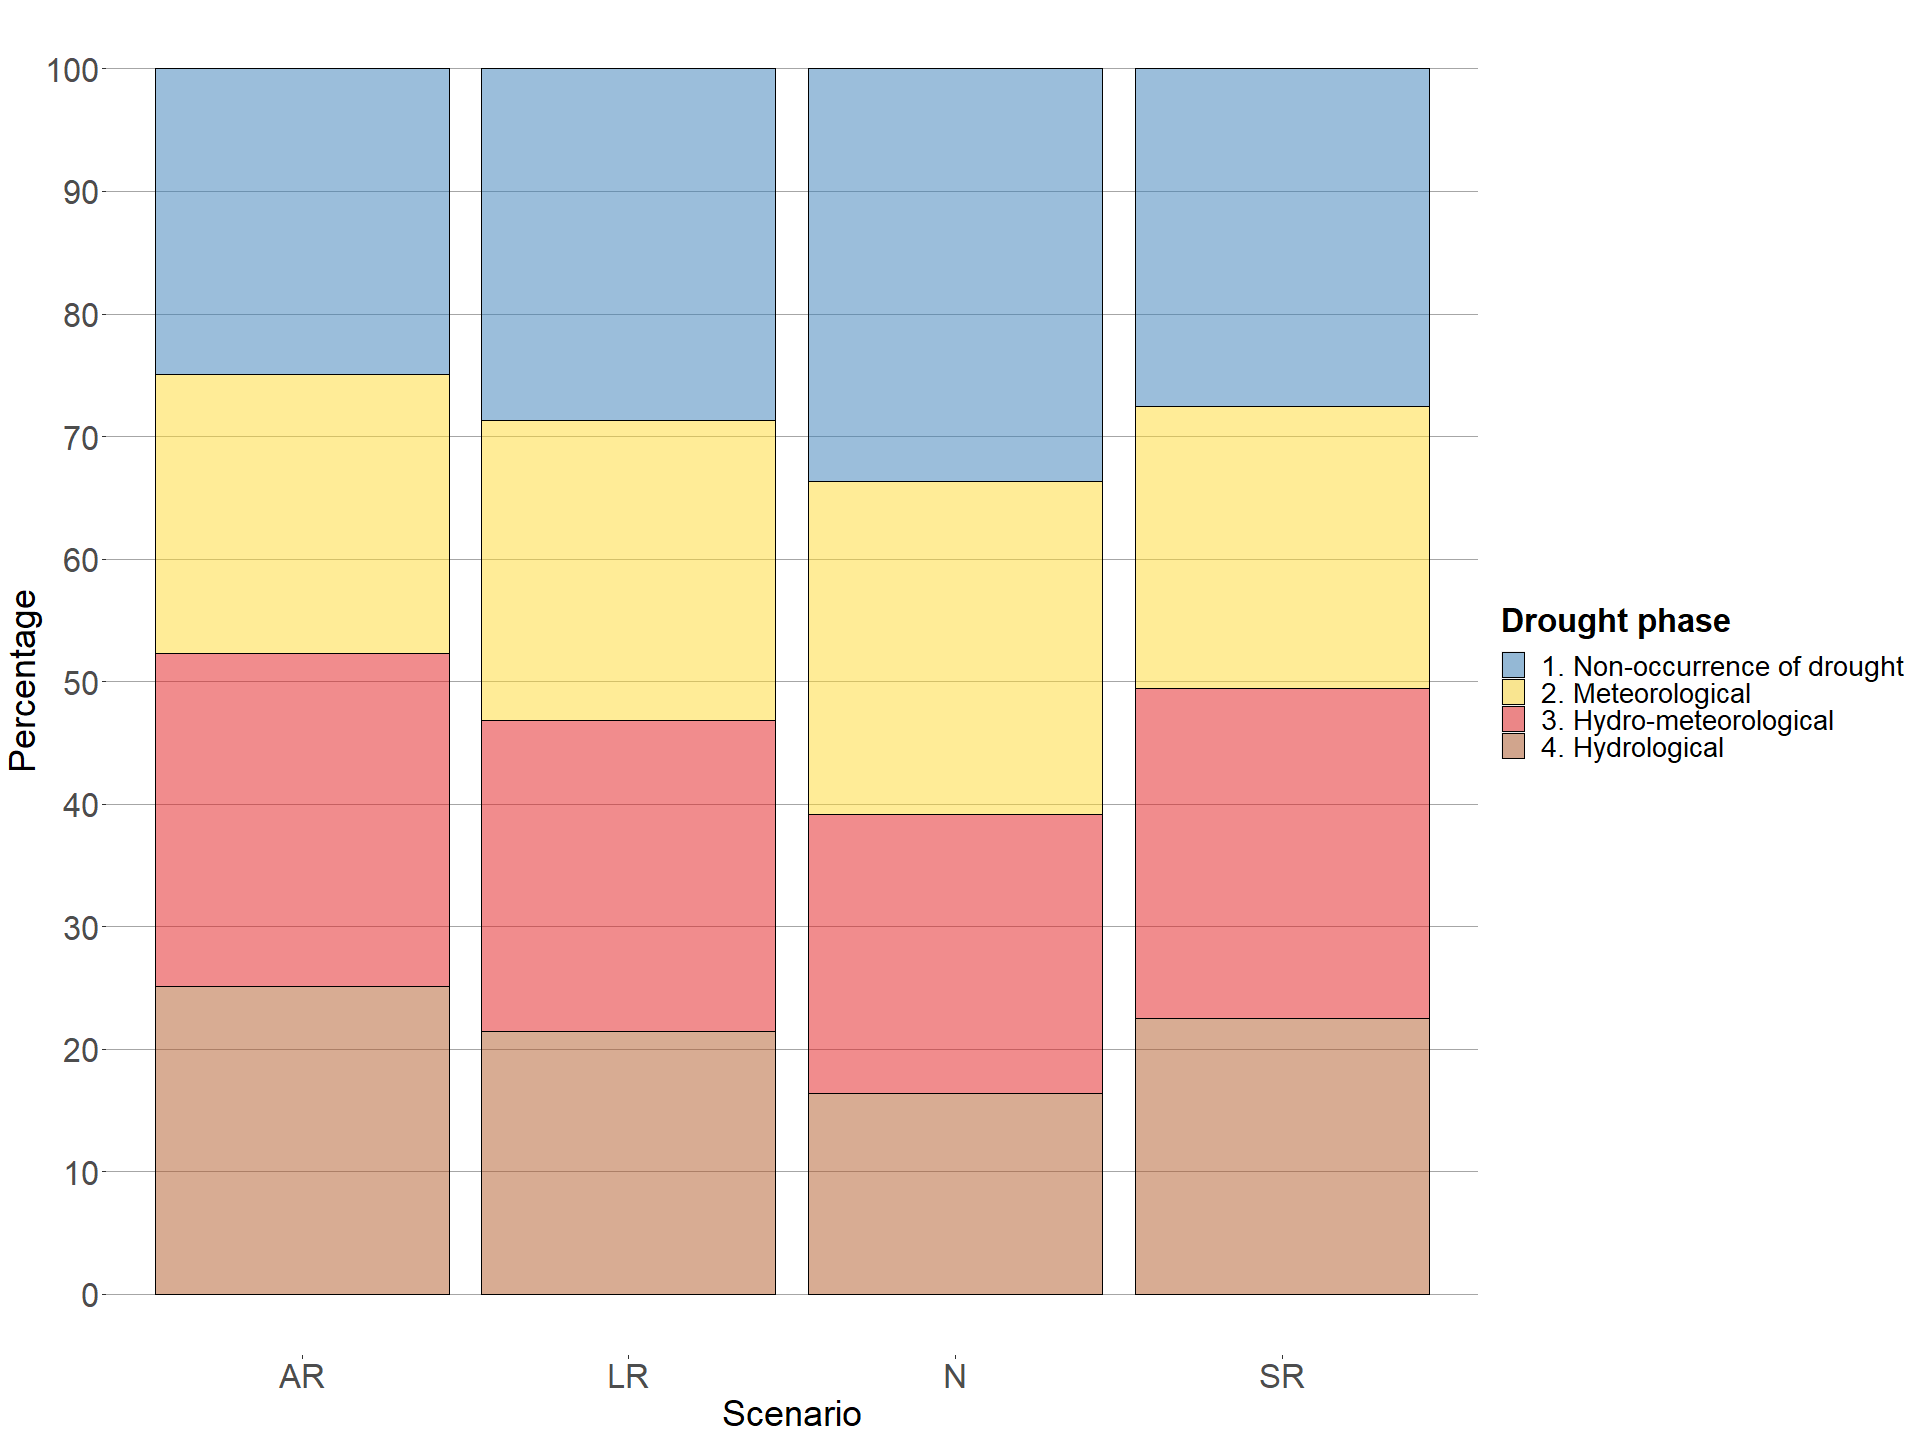
\includegraphics[width=\textwidth]{images/Figure_7.png}
 \caption{Barplot of the drought phases percentages in the four scenarios. Percentage of months in the four drought phases in AR, LR, SR and N scenarios computed for Arrojado Lisboa.}
 \label{fig6}
\end{figure}

%Figure 7
\begin{figure}
 \noindent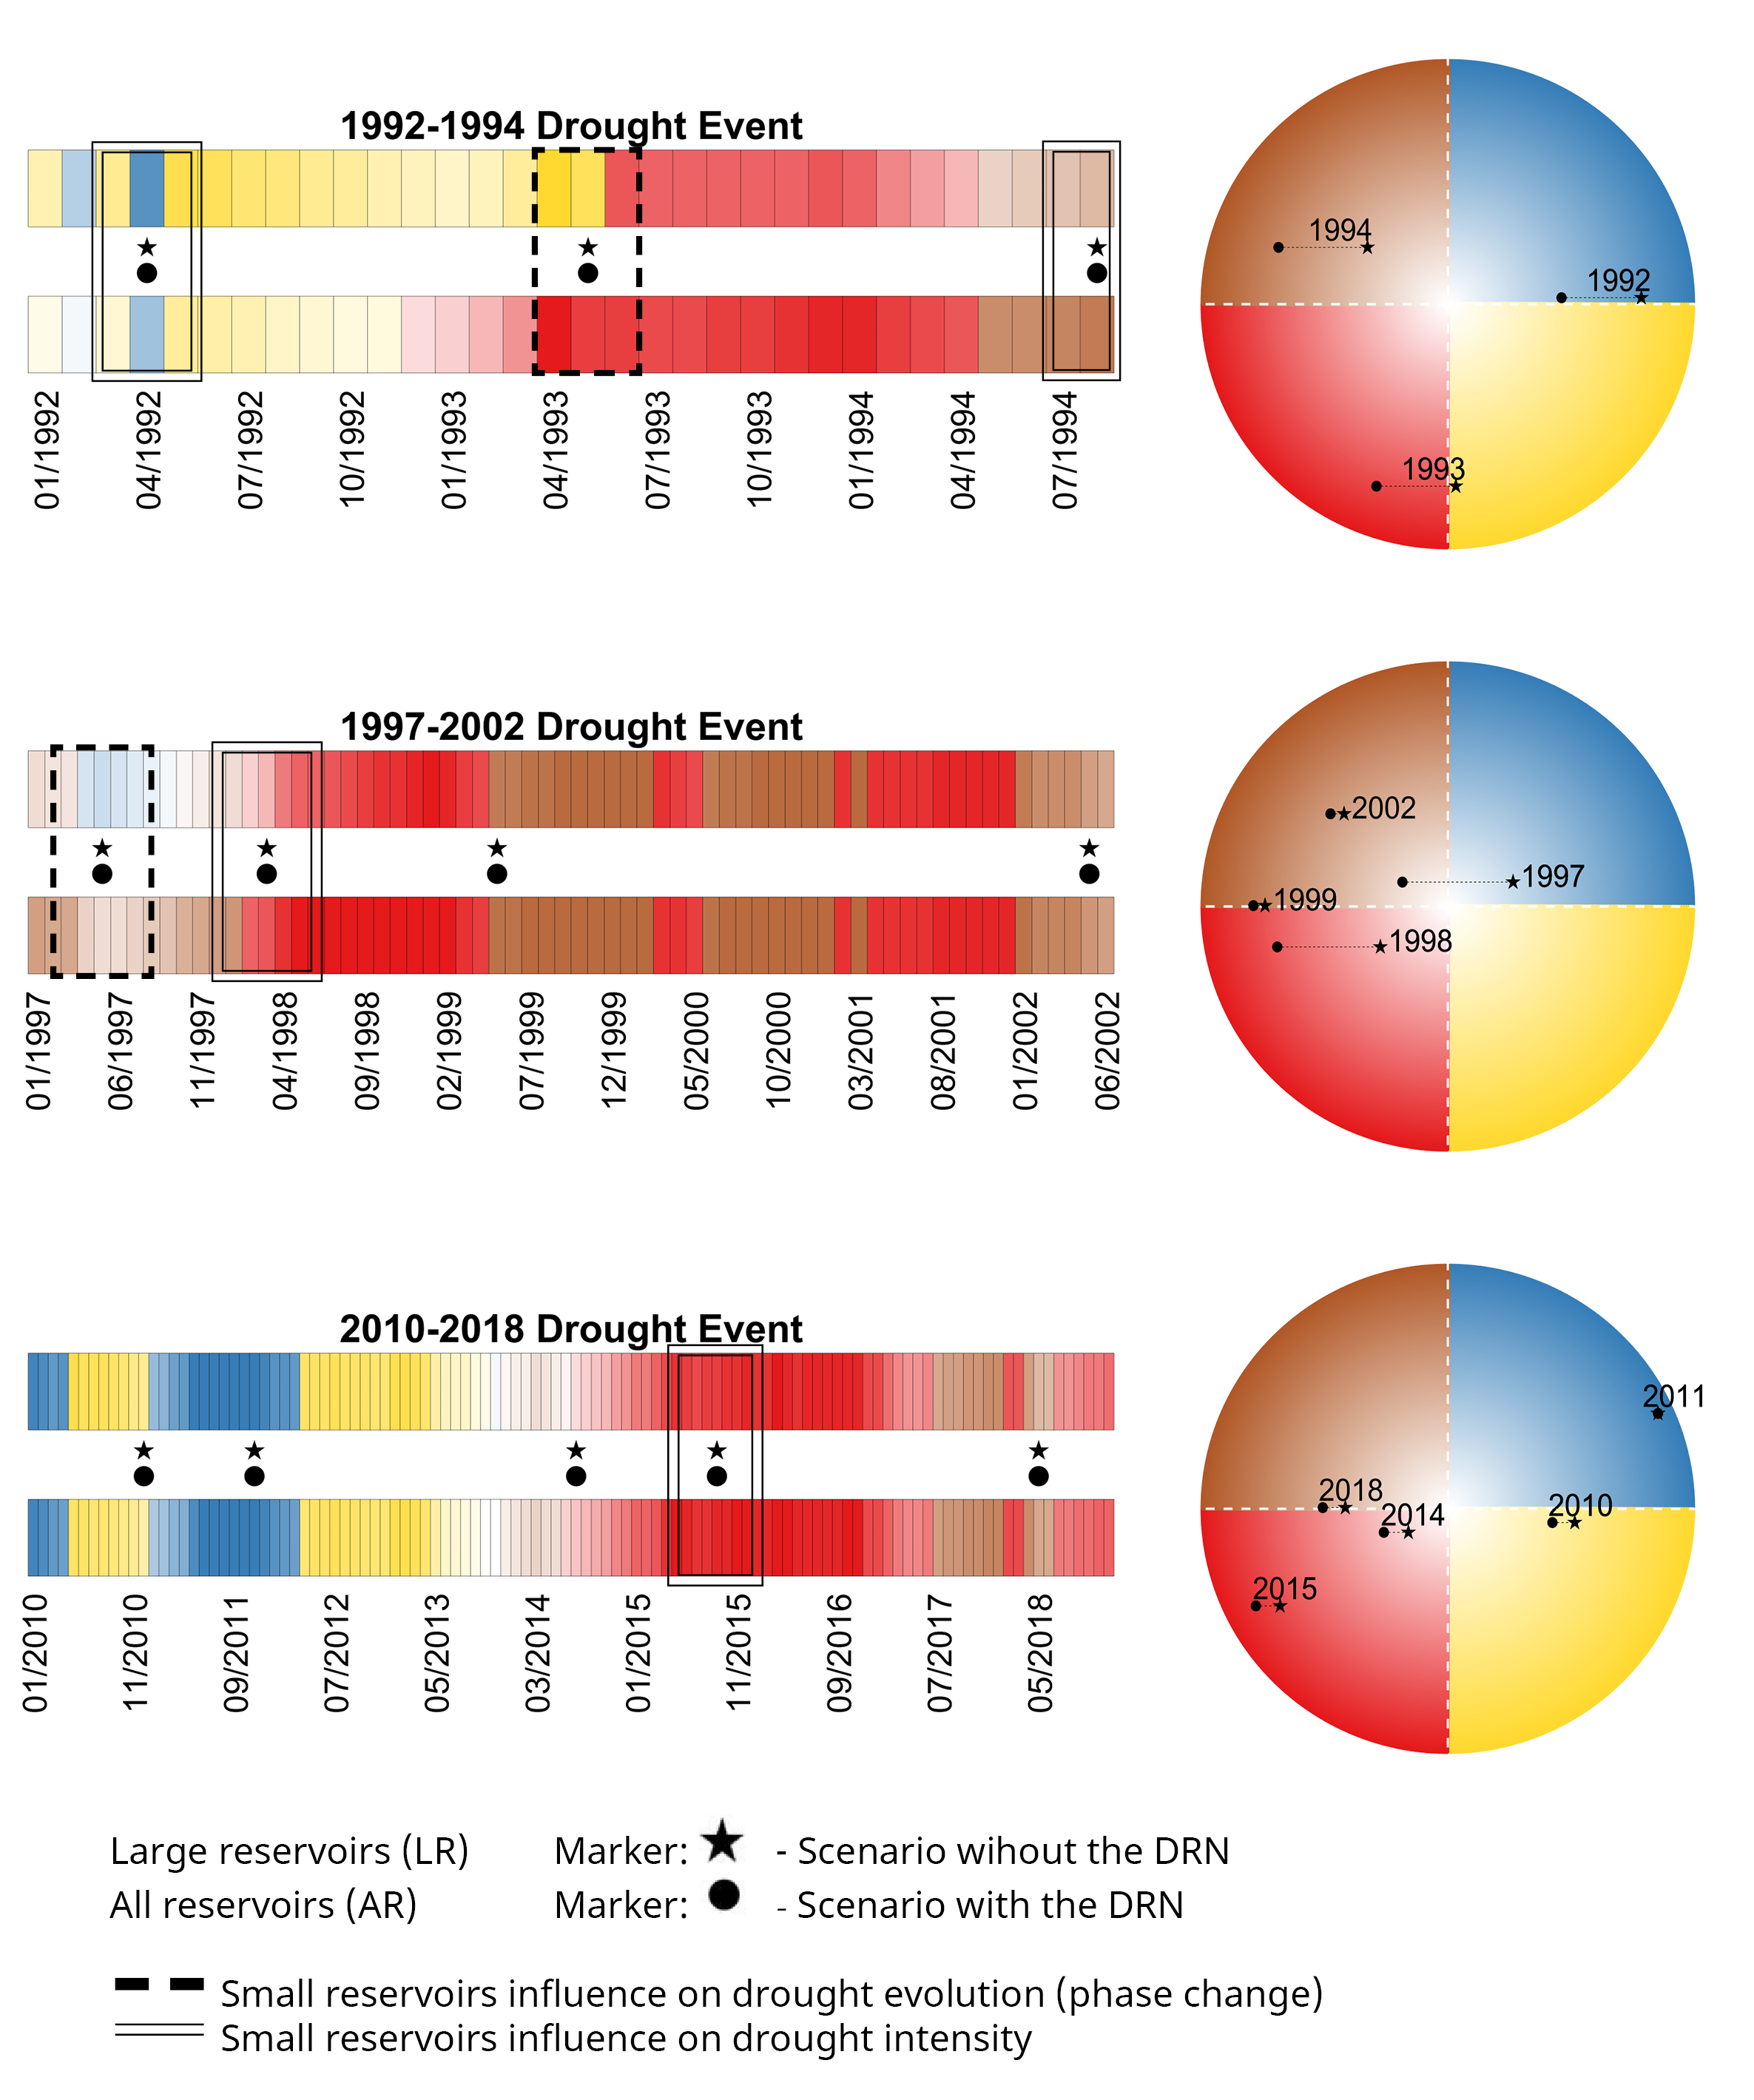
\includegraphics[width=\textwidth]{images/Figure_6.png}
 \caption{Drought Cycle Analysis results for AR and LR, for three distinct drought events. The colors of the monthly-spaced horizontal bars align with the colors in the Drought Wheel. The black circle and star in between the horizontal bars indicate time periods that are indicated inside the Drought wheel. The distance between the circle and the star is the difference between scenarios, showing the impact of the small reservoirs in the DRN on volume deviation.}
 \label{fig7}
\end{figure}

The percentages of months in the 4 drought phases are shown in Figure~\ref{fig6}. The scenarios follow the same pattern across the 4 phases. Without the small reservoirs the percentage of months without droughts increases. The LR scenario presents a lower percentage of months in drought conditions compared to AR: 71\% against 75\%, respectively, which translates to 25 more months in hydrological-related droughts in AR. The scenarios with small reservoirs (AR and SR) have a lower percentage in Phases 1 and 2 (non-occurrence and meteorological drought), and a higher percentage in Phases 3 and 4 compared with N and SR scenarios. Focusing on AR and LR, the months missing from the meteorological drought state moved towards hydro-meteorological droughts (6.8\% increase of Phase 3 in AR), while hydrological droughts extended over periods with non-occurrence of drought (17\% increase of Phase 4 in AR). The result is an overall 12\% increase in hydrological related phases when small reservoirs were present. The increase of hydrological droughts due to the presence of the DRN is enhanced by the absence of large reservoirs: an overall 26\% increase, with 19\% and 38\% in Phase 3 and 4 respectively in SR compared with N. The existence of the DRN thus extends the hydrological related droughts, with a higher increment in the pure hydrological drought, therefore stretching the duration of the drought events.\\
The Drought Cycle Analysis was concentrated in the three most intense drought events. The 1992–1994, 1997–2002, and 2010–2018 drought events are represented in Figure~\ref{fig7} showing the  drought phases for All Reservoirs and Large Reservoirs scenarios. Each month is associated with its color on the wheel, and on the horizontal bars are marked periods in which the influence of the DRN on drought evolution and intensity is particularly visible. In the first event, the AR scenario experiences an early transition towards the hydro-meteorological drought phase (May 1993) and the intensity remains higher until the end of the event. At the beginning of the second event (June 1997) the AR scenario was still in a hydrological drought condition, while the faster recharge in absence of the network (LR) allowed it to avoid a hydrological drought condition. The drought intensity in this first year of the event is considerably higher in the AR scenario, while afterwards they tend to become more similar. In the third event no changes of phase happen, just an increase in intensity in the AR scenario. The existence of the DRN then led to faster transitions towards hydrological drought phases and also increased their intensity.

\subsection{Downstreamness}
%Figure 8
\begin{figure}
 \noindent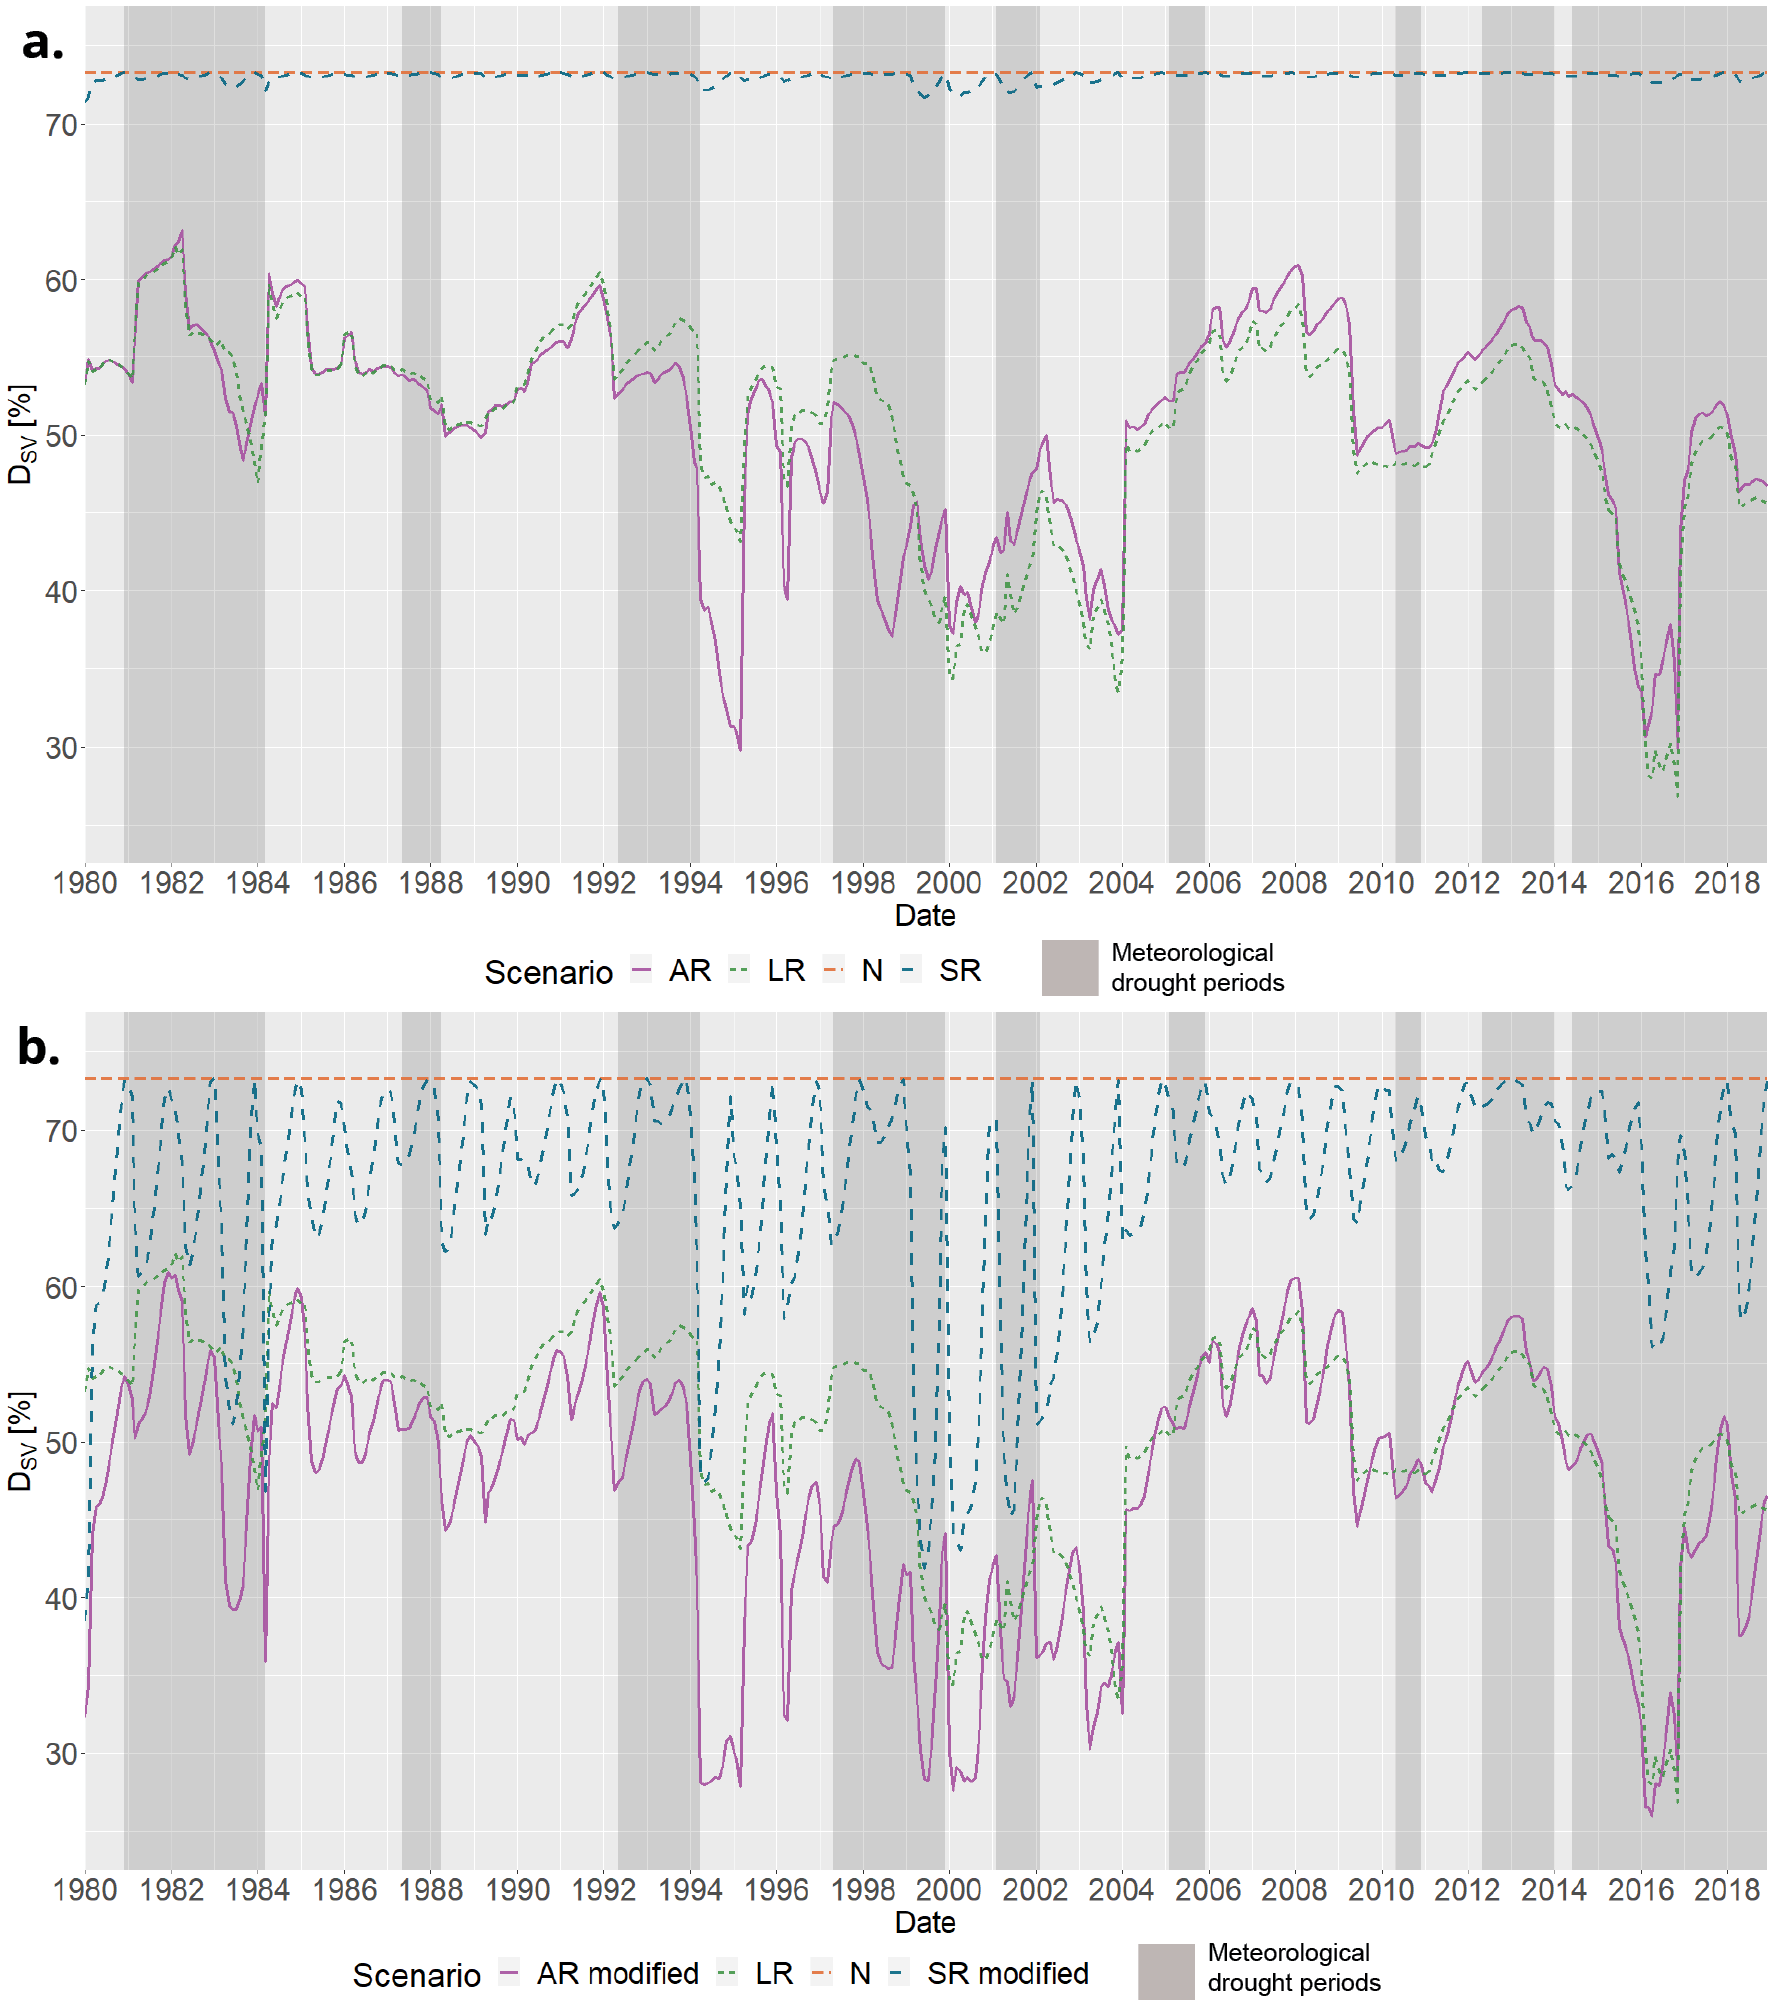
\includegraphics[width=\textwidth]{images/Figure_8.png}
 \caption{Downstreamness of Stored Volume for the four modeled scenarios. In b.) AR and SR scenarios’ $D_{SV}$ are modified by multiplying the stored volume in the DRN by the mean ratio between volume and storage capacity (34\% increase).}
 \label{fig8}
\end{figure}

\textbf{Downstrweamness of storage capacity ($\bm{D_{SC}}$)}

The presence of the small reservoirs network in the AR scenario decreased the downstreamness of storage capacity by 7.76\% on average, compared to LR. The decrease varies from 8.75\% in 1980 to 7.1\% in 2018, due to constructions of new strategic reservoirs which have a high relative weight, decreasing the small reservoirs relative effect in the downstreamness. The most impactful large reservoirs in terms of increased storage capacity were Patu (constructed in 1988, capacity 71.8 $Hm^3$, +3.2\% increase),  Cipoada (1992, 86.1 $Hm^3$, +3.7\%) and Fogareiro (1996, 119 $Hm^3$, + 4.75\%). In terms of $D_{SC}$, 1992 was the most influential year, with 4 reservoirs built for a 4\% decrease in downstreamness with respect to the year before. The single most impactful reservoir in terms of $D_{SC}$ was Pirabibu (2000, 74 $Hm^3$, -2.5\%) followed by Fogareiro (1996, 119 $Hm^3$, -1.7\%). The existence of the small reservoirs network thus moves the potential water availability more upstream than what is permitted by the large reservoirs alone. The construction of strategic reservoirs always decreased the $D_{SC}$, which may suggest an infrastructural planning towards a more diffused storage capacity in the basin.

\textbf{Downstrweamness of stored volume ($\bm{D_{SV}}$)}

The scenarios’ $D_{SV}$ are plotted in Figure~\ref{fig8}. The effect on the stored volume is instead not this clear. For the scenarios without large reservoirs $D_{SV}$’s behavior is similar to the storage capacity, confirming the network’s ability to store water more upstream: in SR the downstreamness of stored volume is lowered by the existence of small reservoirs (0.35\% on average), with a maximum decrease of 2\% in 1999 compared to N. The effect becomes less straightforward reintroducing the large reservoirs. Between 1980 and 2000 the presence of the DRN is associated with an average 3.85\% decrease in $D_{SV}$, peaking at 31\% in 1995. After 2000 the behavior is inverted: water is stored on average 4.6\% more downstream when the small reservoirs are present. Between 1995 and 2000 the volume stored in large reservoirs increased by 10\% with a 4.6\% decrease in $D_{SC}$, and this can be a factor for the inversion. The broad scale effect of the small reservoirs in space is thus limited and influenced by large reservoirs, which have a higher ability to move large quantities of water. The presence of small reservoirs marginally increases the variability of the stored volume distribution in the basin (Coefficient of Variation equal to 13.51\% in LR versus 13.66\% in AR). Without other reservoirs in place, the water would be stored in the strategic reservoirs only, which have less variability in their storage management than small reservoirs. Without large reservoirs this effect is enhanced: the Coefficient of Variation difference between SR and N scenarios is 0.42\%. The presence of the DRN can then increase stored volume variability across the basin, both before (2009) and during a drought event (2016), but the presence of a large reservoir network limits this effect. In all scenarios, $D_{SV}$ is higher than $D_{SC}$ 85\% of the time. As explained in \citeA{VanOel2011} this indicates that most of the time the water is stored more downstream than upstream.\\
The modeled cumulative volume stored in the DRN at each time step is always one order of magnitude lower than the network’s total capacity. It is then possible that the model is underestimating the volume effectively retained in the DRN. To overcome this possibility and explore a condition in which the DRN is able to reach its storage capacity, new $D_{SV}$ for the AR and SR scenarios were obtained by multiplying the stored volume in the DRN by the mean ratio between volume and storage capacity (34\% increase). The result is shown in Figure~\ref{fig8}b. The variability in the new series is increased, and it is more evident the effect of DRN existence: water is stored more upstream by an average of 9\% in SR modified and 7\% in AR modified, confirming how the existence of large reservoirs dampens the DRN effects. In AR, increasing the volume stored in the DRN confirmed that the overall trend of the water distribution in the basin is more dependent on the large reservoirs when these are more present, since the $D_{SV}$ still follows the LR series trend after 2000. At the same time the seasonal trend is more prominent in these scenarios, due to the DRN’ seasonal trend itself being more relevant. The fictional enhancement in the DRN’s stored volume confirmed the observations made on the previous series, both on the increased variability in water distribution and in the higher relative weight that large reservoirs have in determining the trend and where water is allocated.

\section{Discussion}

\subsection{Discussion of findings}
Recent studies came to similar results about the influence of DRN on droughts in time \cite{Rabelo2021,HvanLangen2021,RibeiroNeto2022}. Some results about the influence in space however remain open to discussion: the $D_{SV}$ does not vary significantly without considering the DRN in the AR scenario calculation (RMSE of 0.181 between the two series). In the AR scenario the DRN contributes to 0.26\% of the total stored volume, while strategic reservoirs cover the remaining 99.74\%. However, the volume collected by the small reservoirs in the AR scenario is not able to match the volume increment collected by the strategic reservoirs while the DRN is missing (LR). The modeled cumulative volume effectively retained in the DRN is always one order of magnitude lower than its total storage capacity. This consistent reduction in the water yield could be explained by higher dispersion and transmission losses due to a more diffused network. The higher infiltration and evaporation rates in small reservoirs can also be an important factor of the difference, which in turn are enhanced by the DRN’s highly variable nature \cite{Malveira2012}. However, this could also be explained by an underestimation operated by the model and can be linked to these uncertainties as well as the ones described in Section~\ref{sec:studylim}. In this research the DRN’s retained volume was used to assess the downstreamness of stored volume: to overcome this possible underestimation fictional scenarios with increased volume of the DRN were generated and presented. Future application of the methodology should also consider this issue or assess the uncertainty related to the volume.\\
The downstreamness of stored volume ($D_{SV}$) results in AR and LR scenarios are not completely clear. To provide more details, downstreamness could be computed and analyzed also for each sub-catchment in the Banabuiú basin. This will result in higher resolution on the whole basin, making it possible to describe local and diverse conditions. The different reservoirs’ behavior throughout the basin in relation to the DRN can be analyzed to examine possible differences in the network’s influence between upstream and downstream reservoirs \cite{HvanLangen2021}. This could be also useful to explore a noted pattern: when a meteorological drought happens, the $D_{SV}$ tends towards lower values, thus moving the stored volume upstream.

\subsection{Study limitations}\label{sec:studylim}
In the model’s definition of small reservoirs, smaller reservoirs are assumed to be located upstream of larger ones, which has been based on experience in dryland areas in Brazil and qualitative reasoning form topographic maps \cite{Mamede2018,Guntner2004}. This assumption is an approximation of the real condition, which is a combination of cascade and parallel reservoirs. The connections between small reservoirs are then not fully considered, and this could lead to an underestimation of their effect on hydrological droughts. How much this simplified scheme influences the final results could be estimated by performing a comparison with a more detailed representation of large and small reservoirs as the one performed in \citeA{Rabelo2021}, where it was used to analyze the cumulative impact of small reservoirs on the horizontal hydrological connectivity. Hydrological modeling is defined as one of the best methods to estimate variables of interest as flow and volume in absence of direct measurements \cite{Marahatta2021}. The selection of a model, however, should be based on its adequacy to the task, as it has been done in this research \cite{Addor2019}. WASA-SED hydrological model is feasible and ready to model a dense network of small reservoirs, as it already presents a module specifically for this task. Another promising and widely used large-scale model is MGB-IPH, made available from the Institute of Hydraulic Research of the Federal University of Rio Grande do Sul. Similarly to WASA-SED, MGB-IPH divides the hydrographic basin into small sub-basins, but its adaptability to the task of modeling a DRN hasn’t been proved yet \cite{Collischonn2007,DePaiva2013}. SWAT eco-hydrological model (Soil and Water Assessment Tool) is another candidate for the detailed representation and simulation of large and small reservoirs, in particular in catchments where water extraction and agriculture are relevant (Arnold et al., 2012; \cite{Rabelo2021}).\\
Water withdrawals time series from Arrojado Lisboa are not enough to fully explain the reservoir’s observed volume variations. Other drivers could be involved in periods where withdrawals don’t explain the volume decrease, which is not happening in the modeled simulations. Direct extractions from the reservoirs may be one of these drivers, for example extractions performed through water trucks or by mechanical pumps for households or commercial bottled water \cite{DeLiraAzevedo2017}. These sources of uncertainty in water management could be quantified or estimated, then added to the known withdrawals.\\
Another source of uncertainty comes from the small reservoirs locations and size. The number of small reservoirs has been kept the same across the whole time series, by utilizing the survey made available by FUNCEME \cite{FUNCEME2021}. Small reservoirs without a counterpart in JRC’s Global Surface Water Explorer (procedure explained in \ref{sec:drncap}) were removed from the dataset. It means that approximately 7,000 reservoirs were not modeled and their influence was not estimated. Even though these reservoirs would probably have fallen in the lowest class, it is still likely that their presence would have enhanced the DRN effects. Remote sensing techniques could be used to improve the detection and consideration of reservoirs also throughout the years \cite{RibeiroNeto2022,Pereira2019,Avisse2017,Ogilvie2016}. The model itself introduced uncertainties, as the modeled volume time series can never perfectly reproduce the real world condition, even though the calibration and validation were satisfactory. The procedure to obtain the downstreamness of each small reservoir can introduce uncertainties since the downstreamness value is related to the accuracy of the DEM used as the starting point. In this study, the DEM resolution is 90 m at the equator \cite{CIAT2021}, so it permits an accurate representation of the downstreamness.

\subsection{Further analyses and future studies: cooperation, policies and climate change}
The analyses here conducted can be further applied involving more the Naturalized and Small Reservoirs scenarios. The influence of the hydraulic structures and their operations on drought evolution can then be calculated excluding other influences. For example, the hydrological drought driven only by climate can be obtained from the volume deviation in the N scenario. Then, the hydrological drought driven by small reservoirs can be obtained by subtracting N from SR, the one driven by large reservoirs from LR minus N, and the one driven by the combined effects of large and small reservoirs from AR minus N. In order to explore the evolution through space of the drought phases, the Drought Cycle Analysis could be performed by including the spatial dimension together with the already considered time dimension, in a similar way as Figure~\ref{fig4}b. A visual representation of the basin could be provided, with drought phases and intensities information displayed in the different areas of the basin, for example in each sub-basin.\\
Possibilities are open to further investigate the influence of DRN and to evaluate possible forms of mitigation of its effects. Cooperation between the reservoir operators could be a viable path to reduce the effects of the DRN on the strategic network of reservoirs, and could be investigated in future studies. Evidences in benefits from coordinated reservoir operations are highly documented, addressing optimization of economic, social and environmental issues \cite{Castelletti2008}, flood mitigation \cite{Seibert2014}, or multi-objective and complex international scenarios \cite{Giuliani2021}. Different possibilities arise when dealing with existing infrastructure: operable reservoirs included in the DRN could be used as buffers to collect water from extreme events and then distribute it in higher necessity periods, while the efficiency of some big strategic reservoirs could be questioned and rediscussed. Scenarios of cooperation could be already performed through the WASA-SED model. The operable reservoirs included in the DRN could be fully parameterized and considered as strategic reservoirs, a set of alternatives can then be evaluated defining and testing operational rules. The objectives of the scenario could be to minimize the hydrological drought phases length and to maximize the water distribution across the basin, in order to find a configuration which best fulfills these goals. Policies which improve meaningful public participation may represent a complementary DRN effects mitigation solution to the simulation of the reservoirs operations. Participatory management and plans involving local communities and other stakeholders can improve decision making at the river basin level, finding a balance between the need to decentralize water storage and the evidence that strategic reservoirs provide a more stable option in water storage \cite{Lemos2007,DeLiraAzevedo2017}. A study on the policies and the existing realities in Ceará and in the Banabuiú basin could be useful to better understand how to address the existence and the impacts of the DRN on a more social level. On a last note, climate change is unequivocal and will influence most environmental aspects both in the present, near and distant future \cite{IPCC2021}. Studying which role the DRN can play in this changing context can be important. It has been observed that in the past its existence stretched the duration of hydrological drought periods in strategic reservoirs, and it is presumably that the same will happen in the future if anything changes. On which degree this will happen is uncertain, due to various sources of uncertainty \cite{Hattermann2018,Randall2007}. Studies have already been done on projected climate change scenarios in semiarid areas \cite{Zhao2014,Marengo2020,Marengo2017}, but exploring the impacts of the small reservoirs network in these future contexts can be useful to address the drought preparedness of the region and possible mitigation solutions \cite{Gutierrez2014}.

\section{Conclusions}
In many semi-arid areas small reservoirs are built without regulation nor monitoring, both as a preparedness measure to drought and to respond to the growing water demand \cite{Krol2011,Avisse2017}. They form a dense network, and its combined effects are mainly unexplored. This study shows its effect on drought propagation, exploring both the time and space domains, providing novel information to answer the 22nd question from the 23 “unsolved problems in hydrology” \cite{Bloschl2019}: What are the synergies and tradeoffs between societal goals related to water management?\\
To address the effect of the existence of a DRN on drought evolution, realization of the watershed including and excluding the small reservoirs have been simulated. WASA-SED was the model selected for this task, a semi-distributed hydrological model able to simulate wide semi-arid areas considering both state-controlled strategic reservoirs and networks of diffused reservoirs \cite{Guntner2002,Guntner2004,Mueller2010}. To explore the DRN effects in time the Drought Cycle Analysis was performed, which makes it possible to compare the drought phase and intensity between scenarios \cite{RibeiroNeto2022}. To explore the effects in space, the Downstreamness Analysis was performed, assessing the changes in the distribution of the storage capacity and the stored volume throughout the basin \cite{VanOel2018}. Interesting aspects on the role of the DRN emerge from the results of the Drought Cycle Analysis and the Downstreamness analysis. In time, the presence of the network of small reservoirs accelerates the transition towards hydrological drought phases by 20\% on average and slows down the recharge period in strategic reservoirs by 25\%. This translates in a 7\% increase in hydro-meteorological drought periods and a 17\% increase in hydrological drought periods, for a combined 12\% increase in hydrological related droughts. These influences were proven stronger when big strategic reservoirs are missing, with a 26\% increase in hydrological related droughts. The presence of a large reservoir network acts then as an attenuator of the DRN effects in time. DRN may enhance droughts' impacts when the basin is already in a dry condition. When large reservoirs are already in a depletion condition, the effect of the DRN is enhanced: having a better knowledge of this phenomenon may help the implementation of short term drought preparedness measures when the reservoirs are below a threshold (e.g. 75\% of the maximum capacity). In space, the DRN existence leads to an average increase of 8\% in upstream distribution of the storage capacity. When large reservoirs are missing, the DRN permits to store more volume upstream, reducing the $D_{SV}$. The low and highly variable actual stored volume retained in small reservoirs, however, results in a negligible direct influence on the downstreamness of stored volume when strategic reservoirs are present. This leads the water distribution in the basin to be more dependent on large reservoirs relative conditions. The methodology followed has been proved successful to permit an assessment of the DRN influence on the hydrological drought evolution in a basin in time. Interesting information about the DRN’s effect in the storage capacity and stored volume spatial variation, although the latter results become less interpretable when large reservoirs are present. There is however the possibility that the DRN’s retained volume is underestimated and although this doesn’t affect the outcomes of this research the underestimation should be tested and eventually corrected in future applications.\\
The role of the DRN on the evolution of droughts is multifaceted: in time it increases the incidence and the intensity of hydrological drought phases; in space it increases the upstream storage capacity while it may lead downstream large reservoirs to store less water, leading them to potentially higher drought impacts. It is then useful to further explore the relationships between the effects in time and space, deepening the knowledge about the influences of the DRN and the causes behind the effects here identified through future studies and analyses. The results may help the implementation of drought preparedness and adaptation measures in the Banabuiú basin and in other similar conditions both in North-East Brazil and other semi-arid areas.

%%% End of body of article

%%%%%%%%%%%%%%%%%%%%%%%%%%%%%%%%
%% Optional Appendix goes here
%
% The \appendix command resets counters and redefines section heads
%
% After typing \appendix
%
%\section{Here Is Appendix Title}
% will show
% A: Here Is Appendix Title
%
%\appendix
%\section{Here is a sample appendix}

\newpage
\appendix
\section{Additional table}

%Table A
\begin{table}
 \caption{Appendix: List of centralized reservoirs, with storage capacity and upstream catchment. The table is ordered by decreasing storage capacity. Information retrieved from FUNCEME database \url{funceme.br/hidro-ce-zend/}.}\label{tabA}
 \centering
 \begin{tabular}{c c c c}
 \hline
  Name  & Year constructed & Storage capacity & Drainage area\\
  & & [$Hm^3$] & [$km^2$]\\
 \hline
Arrojado Lisboa 	& 1966 &	 14,221	& 1600\\
Pedras Brancas	& 1978	& 1,937 &	434\\
Cedro			& 1906	& 206 &	126\\
Fogareiro 		& 1996	 & 5,111 & 	119\\
Cipoada			& 1992	& 351 &	86.1\\
Pirabibu			& 2000	& 503	& 74\\
Patu	 			& 1988	& 995	& 71.8\\
Poço do Barro	& 1956	 & 374 & 52\\
Serafim Dias 	& 1995 &	1,630 &	43\\
Umari			& 2011	& 975	& 30\\
Sao Jose II		& 1992	& 185	& 29.1\\
Vieirão			& 1988	& 400 &	21\\
Trapiá II 		& 1992 & 	129 &	18.2\\
Curral Velho	 	& 2007 & 	79 & 	12.2\\
Monsenhor Tabosa & 1998 & 77 &	12.1\\
Quixeramobim 	& 1966 & 7,021 &	7.88\\
Sao José I		& 1988 & 	188 & 	767\\
Capitão Mor		& 1988	& 110 &	6\\
Jatobá 			& 1997 &	40	& 1.07\\
 \hline
 \end{tabular}
\end{table}

%%%%%%%%%%%%%%%%%%%%%%%%%%%%%%%%%%%%%%%%%%%%%%%%%%%%%%%%%%%%%%%%
%
% Optional Glossary, Notation or Acronym section goes here:

%%%%%%%%%%%%%%
% Acronyms
   \begin{acronyms}
   \acro{AR, LR, SR, N}
   All Reservoirs, Large Reservoirs, Small Reservoirs and Naturalized scenarios generated with WASA-SED model. Explanation in Section~\ref{sec:scenarios}.
   \acro{DEM}
   Digital Elevation Model. 3D representation of elevation data to represent terrain or overlaying objects.
   \acro{DRN}
   Dense Reservoir Network. A great number of small reservoirs creating a network.
   \acro{$\bm{D_{SC}}$, $\bm{D_{SV}}$}
   Downstreamness of Storage Capacity and Stored Volume, respectively. Explanation in Section~\ref{sec:dwn}.
   \end{acronyms}

\section{Open research}

\textbf{Data availability statement}\\
The DEM used for the downstreamness analysis was downloaded through CGIAR’ SRTM database \cite{CIAT2021}. The location of the small unmonitored reservoirs identified by FUNCEME, the meteorological observations (precipitation, temperature, humidity and radiation) and the hydrological observations (strategic reservoirs volumes and releases) are available at \url{github.com/paolchol/DRN-analysis}.\\

\textbf{Software availability statement}\\
The WASA-SED source code is available at \url{github.com/TillF/WASA-SED}, the calibrated model used here is available at \url{github.com/paolchol/DRN-analysis} in the WASA-SED folder. The user guide is available at \url{tillf.github.io/WASA-SED/}. The R and Matlab code used to perform all the operations and figures is provided at \url{github.com/paolchol/DRN-analysis}.

%AGU requires an Availability Statement for the underlying data needed to understand, evaluate, and build upon the reported research at the time of peer review and publication.

%Authors should include an Availability Statement for the software that has a significant impact on the research. Details and templates are in the Availability Statement section of the Data and Software for Authors Guidance: \url{https://www.agu.org/Publish-with-AGU/Publish/Author-Resources/Data-and-Software-for-Authors#availability}

%It is important to cite individual datasets in this section and, and they must be included in your bibliography. Please use the type field in your bibtex file to specify the type of data cited. Options include [Dataset], [Software], [ComputationalNotebook], [Collection].
%Example:
%
%@misc{https://doi.org/10.7283/633e-1497,
%  doi = {10.7283/633E-1497},
%  url = {https://www.unavco.org/data/doi/10.7283/633E-1497},
%  author = {de Zeeuw-van Dalfsen, Elske and Sleeman, Reinoud},
%  title = {KNMI Dutch Antilles GPS Network - SAB1-St_Johns_Saba_NA P.S.},
%  publisher = {UNAVCO, Inc.},
%  year = {2019},
%  type = {dataset}
%}

\acknowledgments
This work is part of the Joint SDG Research Initiative with project number W07.30318.016, which is (partly) financed by the Dutch Research Council (NWO) and the Interdisciplinary Research and Education Fund (INREF) of Wageningen University, the Netherlands.
\clearpage

%% ------------------------------------------------------------------------ %%
%% References and Citations

%%%%%%%%%%%%%%%%%%%%%%%%%%%%%%%%%%%%%%%%%%%%%%%
%
% \bibliography{<name of your .bib file>} don't specify the file extension
%
% don't specify bibliographystyle

% In the References section, cite the data/software described in the Availability Statement (this includes primary and processed data used for your research). For details on data/software citation as well as examples, see the Data & Software Citation section of the Data & Software for Authors guidance
% https://www.agu.org/Publish-with-AGU/Publish/Author-Resources/Data-and-Software-for-Authors#citation

%%%%%%%%%%%%%%%%%%%%%%%%%%%%%%%%%%%%%%%%%%%%%%%

\bibliography{bibliography}

%Reference citation instructions and examples:
%
% Please use ONLY \cite and \citeA for reference citations.
% \cite for parenthetical references
% ...as shown in recent studies (Simpson et al., 2019)
% \citeA for in-text citations
% ...Simpson et al. (2019) have shown...
%
%
%...as shown by \citeA{jskilby}.
%...as shown by \citeA{lewin76}, \citeA{carson86}, \citeA{bartoldy02}, and \citeA{rinaldi03}.
%...has been shown \cite{jskilbye}.
%...has been shown \cite{lewin76,carson86,bartoldy02,rinaldi03}.
%... \cite <i.e.>[]{lewin76,carson86,bartoldy02,rinaldi03}.
%...has been shown by \cite <e.g.,>[and others]{lewin76}.
%
% apacite uses < > for prenotes and [ ] for postnotes
% DO NOT use other cite commands (e.g., \citet, \citep, \citeyear, \citealp, etc.).
% \nocite is okay to use to add references from your Supporting Information
%

\end{document}
